\chapter{Ising a la Samuel}
\section{Grassmann variables}


\newcommand{\mode}{flavor }
\newcommand{\modes}{flavors }
\newcommand{\hdag}[1]{h^{x}_{#1}}
\newcommand{\vdag}[1]{v^{x}_{#1}}
\newcommand{\hnag}[1]{h^{o}_{#1}}
\newcommand{\vnag}[1]{v^{o}_{#1}}
\newcommand{\Hdag}[1]{H^{x}_{#1}}
\newcommand{\Vdag}[1]{V^{x}_{#1}}
\newcommand{\Hnag}[1]{H^{o}_{#1}}
\newcommand{\Vnag}[1]{V^{o}_{#1}}

\newcommand{\cP}{{\cal P}}
\newcommand{\sign}[1]{\text{sgn}\left\{#1\right\}}



%\newcommand{\hdag}[1]{h^{\dagger}_{#1}}
%\newcommand{\vdag}[1]{v^{\dagger}_{#1}}
%\newcommand{\hnag}[1]{h^{\phantom{\dagger}}_{#1}}
%\newcommand{\vnag}[1]{v^{\phantom{\dagger}}_{#1}}

\renewcommand{\xx}[1]{\boldsymbol  x_{#1}}
\newcommand{\ex}{\boldsymbol  e_{x}}
\newcommand{\ey}{\boldsymbol  e_{y}}

\newcommand{\Dep}{{\cal D}_{\eta \psi}}
\newcommand{\Dept}{\tilde {\cal D}_{\eta \psi}}
\newcommand{\Depx}{{\cal D}_{\eta \psi}^{\canceledk{I},\canceledk{J}}}
\newcommand{\Deta}{{\cal D}_{\eta}}
\newcommand{\Detax}{{\cal D}_{\eta}^{\canceledk{I}}}
\newcommand{\Detat}{\tilde {\cal D}_{\eta}}
\newcommand{\Dxi}{{\cal D}_{\xi}}

\newcommand{\Int}{\int\ldots\int}
\newcommand{\Disingi}{{\cal D}_{hv}}
\newcommand{\Pf}[1]{\text{Pf}\left(#1\right)}
\newcommand{\Det}[1]{\text{det}\left(#1\right)}

\newcommand{\set}[2]{\left\{#1_{1},#1_{2},\ldots,#1_{#2}\right\}}
\newcommand{\pairset}[3]{\left\{(#1_{1},#2_{1}),(#1_{2},#2_{2})\ldots,(#1_{#3},#2_{#3})\right\}}

\newcommand{\Set}[2]{\left\{#1_{l}\right\}_{l=1:#2}}
\newcommand{\Pairset}[3]{\left\{(#1_{l},#2_{l})\right\}_{l=1:#3}}



\newcommand{\compset}[3]{#1_{1} #2 #1_{2} #2 \ldots #2 #1_{#3}}

\newcommand{\setprod}[4]{#1_{#2_{1}#3_{1}}\;#1_{#2_{2}#3_{2}}\;\ldots\;  #1_{#2_{#4}#3_{#4}}}
\newcommand{\Setprod}[4]{\prod_{l=1}^{#4}\;#1_{#2_{l}#3_{l}}}


To allow for all elements for admissible graphs we introduce per site 4 
Grassmann variables, two for each direction
$\hdag{i},\hnag{i},\vdag{i},\vnag{i}$, where the first two are for the horizontal direction
and the second two for vertical direction. These are 4 independent variables. Let $\eta $ stand for one of theses variables, then they fulfill
%
\begin{align*}
\int d \eta  &= 0\; \\
\int d \eta  \eta &= 1\\
\eta^{2} &= 0
\end{align*}
%
%
We introduced the trace ($\text{tr}$), which means
%
\begin{subequations}\label{eq:Disingi}
\begin{align}
\tr {f(\{\hdag{i},\hnag{i},\vdag{i},\vnag{i}\})} &= \Int \Disingi\;f(\{\hdag{i},\hnag{i},\vdag{i},\vnag{i}\})\\
\Disingi &= \prod_{i}   d\hdag{i} d \hnag{i}, d\vdag{i},d \vnag{i}
\end{align}
\end{subequations}
%
In particular for a single pair of GV at one site we have
%
\begin{align}
\int\int d \hdag{i} d \hnag{i}  \hnag{i} \hdag{i} &=
\underbrace{
\int d \hdag{i} \hdag{i}
}_{\color{blue} = 1} \underbrace{
\int d \hnag{i}  \hnag{i} 
}_{\color{blue} = 1} = 1\;,
\end{align}
%
but
%
\begin{align}
\int\int d \hdag{i} d \hnag{i}   \hdag{i} \hnag{i}&= -
\underbrace{
\int d \hdag{i} \hdag{i}
}_{\color{blue} = 1} \underbrace{
\int d \hnag{i}  \hnag{i} 
}_{\color{blue} = 1} = -1\;.
\end{align}
%
Obviously, at each site all four GVs have to be present, otherwise the trace over all GVs vanishes.
\clearpage 
We introduce the following graphical meaning for the GV
\begin{figure}[h]
\begin{center}
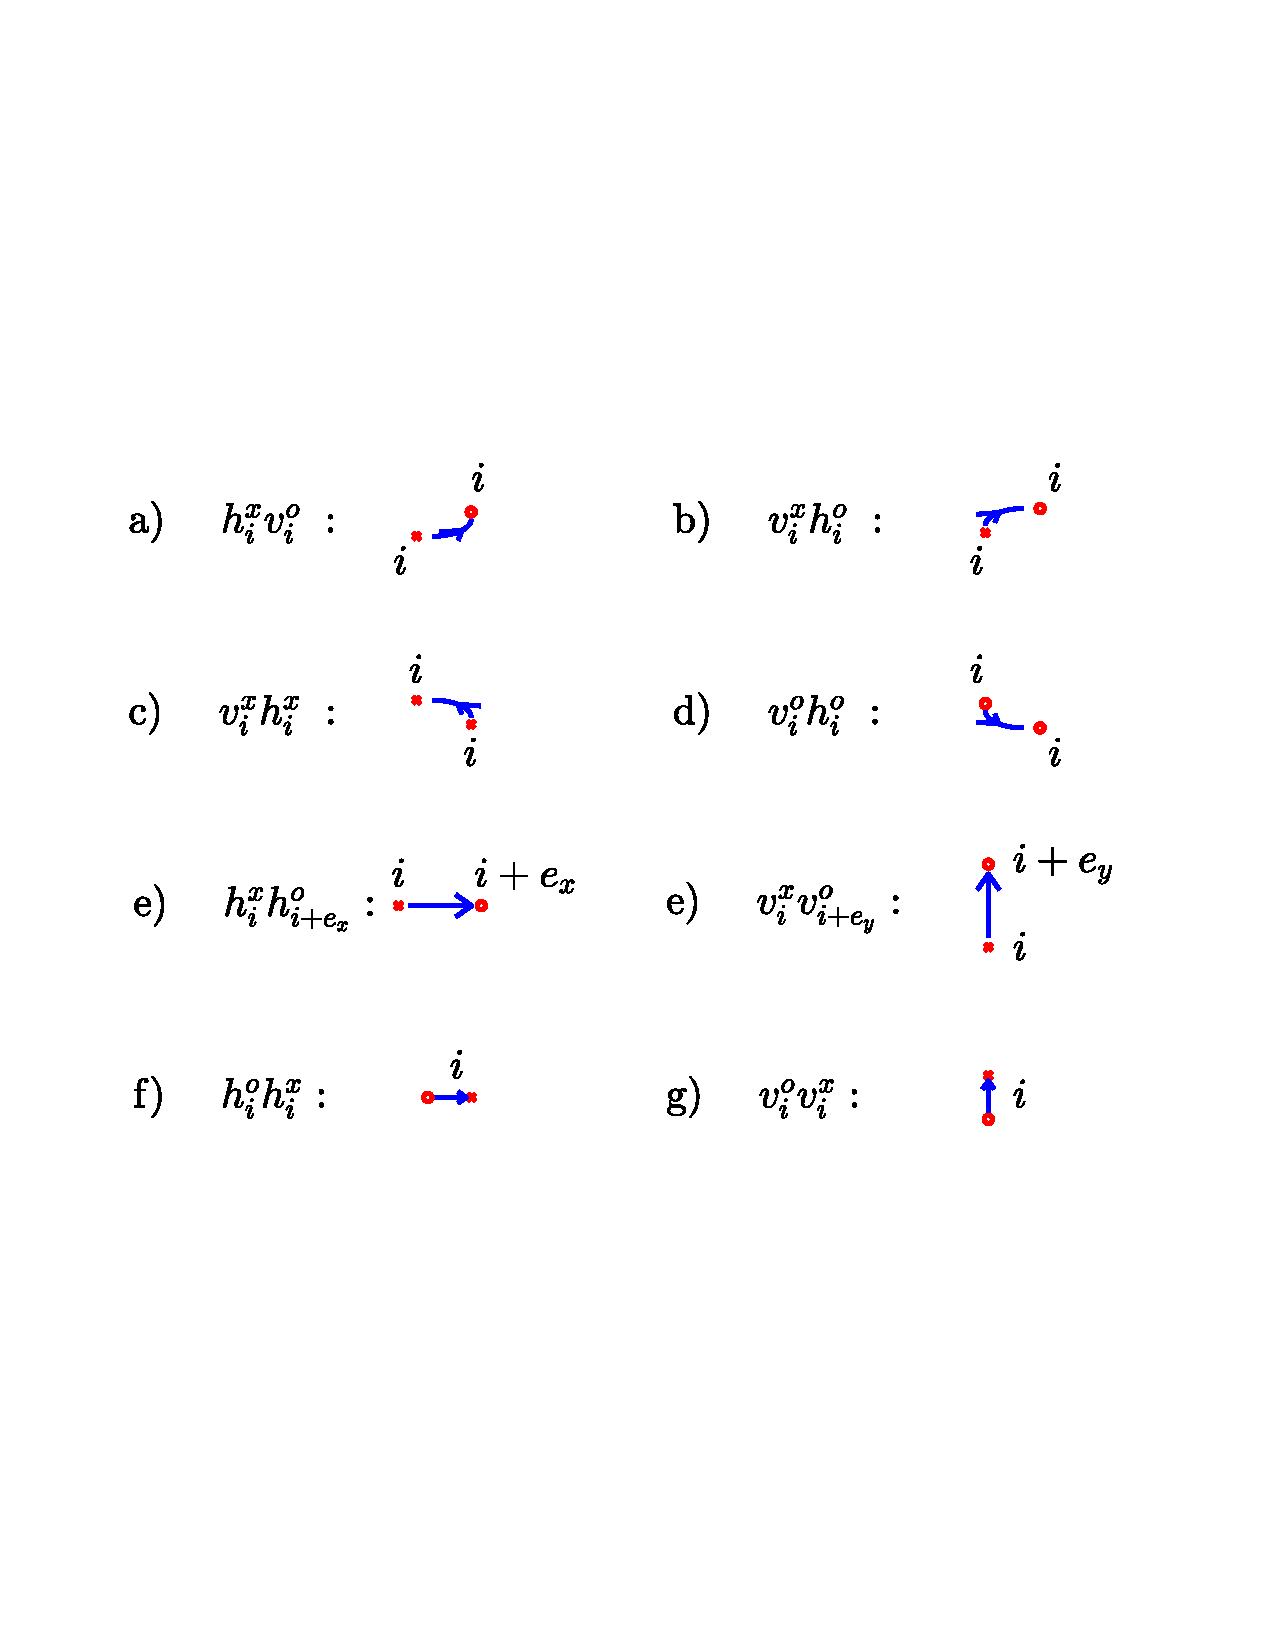
\includegraphics[width=10cm]{GV_pairs}
\caption{{\it The 6 GV-pairs that form the graph elements.}\label{fig:GV_pairs}}
\end{center}
\end{figure}
%

Then we introduce an  action with theses elements
%

\begin{subequations}\label{eq:}
\begin{align}
A &= A_\text{bonds}  + A_\text{corners}  + A_\text{monomers}\\
A_\text{bonds} &= t \sum_{i} \bigg( \hdag{\xx{i}} \hnag{\xx{i}+\ex }
+ \vdag{\xx{i}} \vnag{\xx{i}+\ey}\bigg)\\
A_\text{corners} &=  -\sum_{i} \bigg(\hdag{\xx{i}} \vnag{\xx{i}}+\vdag{\xx{i}} \hnag{\xx{i}}
+\vdag{\xx{i}} \hdag{\xx{i}} 
+\vnag{\xx{i}} \hnag{\xx{i}} 
\bigg)\\
A_\text{monomers} &=  -\sum_{i} \big(\hnag{\xx{i}}\hdag{\xx{i}}
+\vnag{\xx{i}} \vdag{\xx{i}}\big) \\
A&=\sum_{i=1}^{N}  \sum_{\nu=1}^{n_{i}} P_{i}^{(\nu)}
\end{align}
\end{subequations}
%
These elements are depicted in figure \ref{fig:GV_pairs}.
The reason for the minus signs will be clarified later on.
We can then define a kind of partition function
%
\begin{align*}
Z &= \text{tr} e^{A}\;.
\end{align*}
%
We will show in the sequel that 
%
\begin{align*}
\sum_{G} t^{N_{e}(G)} &= (-1)^{N} Z\;.
\end{align*}
%
Since we have a quadratic action in the GVs, we can compute the partition function analytically.
Due to the Grassmannian properties, the pair-variables fullfill $P^{2}=0$.
When expanding $e^{A}$ we, therefore, obtain
%
%
\begin{align*}
e^{A} &= \prod_{i=1}^{N}  \prod_{\nu=1}^{n_{i}} \big(1 + P_{i}^{(\nu)}\big)\;.
\end{align*}
%
Each GV-pair is of the form
%
\begin{align*}
\eta_{i_{1}}^{\alpha_{1}}\eta_{i_{2}}^{\alpha_{2}}\;,
\end{align*}
%
where the lower index stand for the site  and
the upper (type-)index combines the direction $\{h,v\}$ and the \mode $\{x,o\}$.
So we can suitably combine the the GV-pairs $P_{i}^{(\nu)} $. In doing so, we 
have to keep in mind that  each variable for site $i$, i.e.   
$\{\hdag{\xx{i}},\hnag{\xx{i}},\vdag{\xx{i}},\vnag{\xx{i}} \}$ has to occur once and  only once. 



The graphical elements, required to form admitted graphs, are depicted in 
figure \ref{fig:combinations}.
%
\begin{figure}[h]
\begin{center}
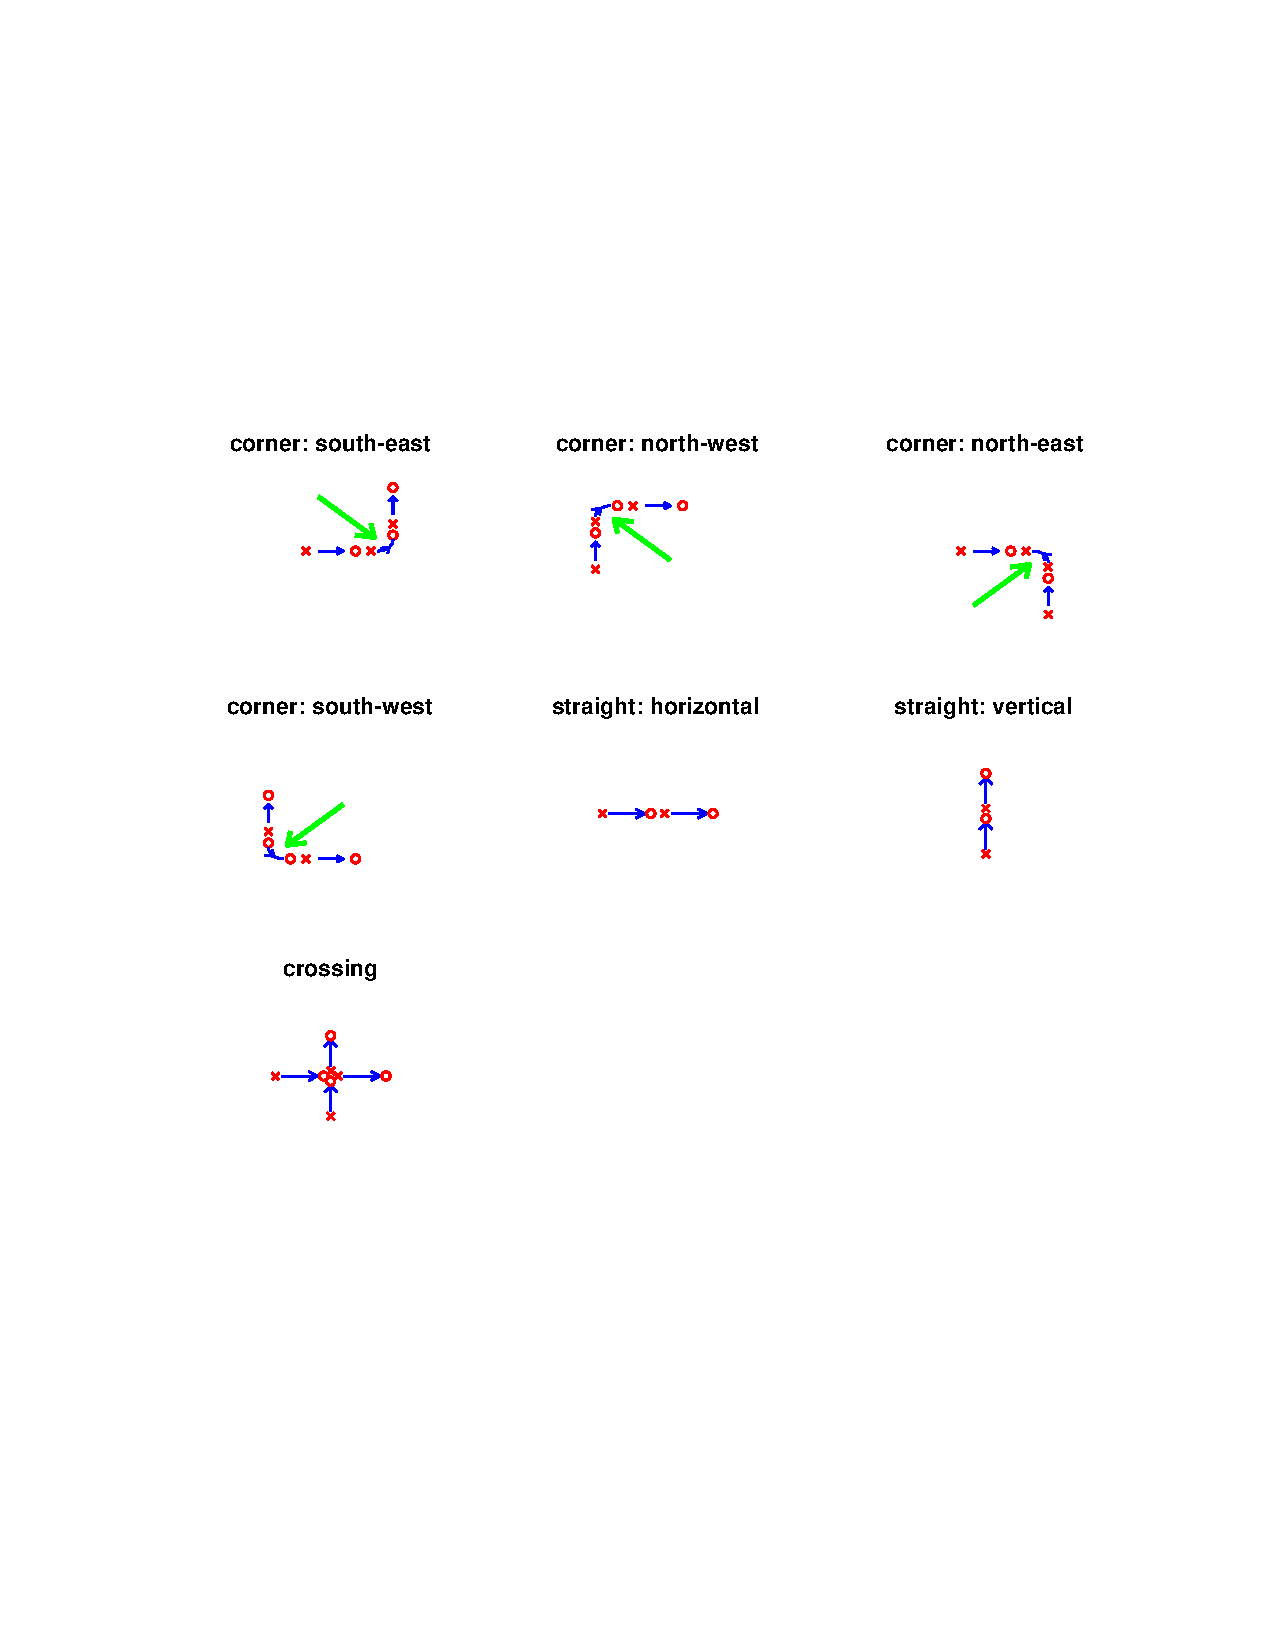
\includegraphics[width=12cm]{path_elements}
\caption{{\it All possible combinations of GV-pairs at one site. Monomers that form empty sites are omitted, as well as monomers, that are needed to complete the straight lines. The elements in these subfigures are the building blocks needed   to form all possible graphs.}\label{fig:combinations}}
\end{center}
\end{figure}
%
These elements are all that is required to form all admitted graphs; and due to the 
Grassmannian properties each graph is generated exactly once. Hence, we have essentially
%
\begin{align*}
\text{tr}\bigg\{ e^{A} \bigg\} &= \sum_{G} \text{sign}(G) t^{N_{e}(G)}\;.
\end{align*}
%
The  factors $t$ are correctly included since each bond is associated with a factor $t$.
We still need to make sure that each admitted graph has the correct sign.
In addition, to the sites that have lines attached to them,
we also need to ensure that empty site are included correctly, i.e. they should only multiply
a factor 1 to each graph.

\subsection{Monomers}
 
The monomers add missing variables, either for empty sites, or those not used  for building the graphs. 

Empty sites can be formed by a monomer pair for the horizontal and one for the vertical
direction, i.e.
%
\begin{align*}
\hnag{\xx{i}} \hdag{\xx{i}}\vnag{\xx{i}}\vdag{\xx{i}}
\end{align*}
%
and the trace gives 
%
\begin{align*}
\underbrace{
\iint d \hdag{\xx{i}} d \hnag{\xx{i}}\hnag{\xx{i}} \hdag{\xx{i}}
}_{\color{blue} = 1}
\cdot\underbrace{
\iint d \vdag{\xx{i}} d \vnag{\xx{i}} \vnag{\xx{i}}\vdag{\xx{i}} 
}_{\color{blue} = 1}&= 1\;.
\end{align*}
%
Also if we include the minus sign in the action, the contribution is $+1$, as the we have $(-1)^{2}$.
Since all GVs at site $i$ are involved, no other GV-pair can occur at site $i$, if there are already the two monomer pairs. 
Alternatively, the product of the GVs of corner a) and b) or  the GVs of corner c) and d)   provide all GVs for site i as well. That yields
%
\begin{align*}
a) \cdot   b) &= \hdag{\xx{i}}\vnag{\xx{i}} \vdag{\xx{i}} \hnag{\xx{i}} =- \hdag{\xx{i}} \hnag{\xx{i}}  \vdag{\xx{i}}\vnag{\xx{i}} 
\end{align*}
%
and the integral gives $-1$. or
\begin{align*}
c) \cdot  d) &=\vdag{\xx{i}}  \hdag{\xx{i}}\vnag{\xx{i}}  \hnag{\xx{i}} =- \hdag{\xx{i}} \hnag{\xx{i}}  \vdag{\xx{i}}\vnag{\xx{i}} \;,
\end{align*}
which also gives $-1$ after the integral.
These 3 terms have to be added, as they all yield an empty site. \blue{So the total weight of an empty site is $-1$}


\begin{figure}[h]
\begin{center}
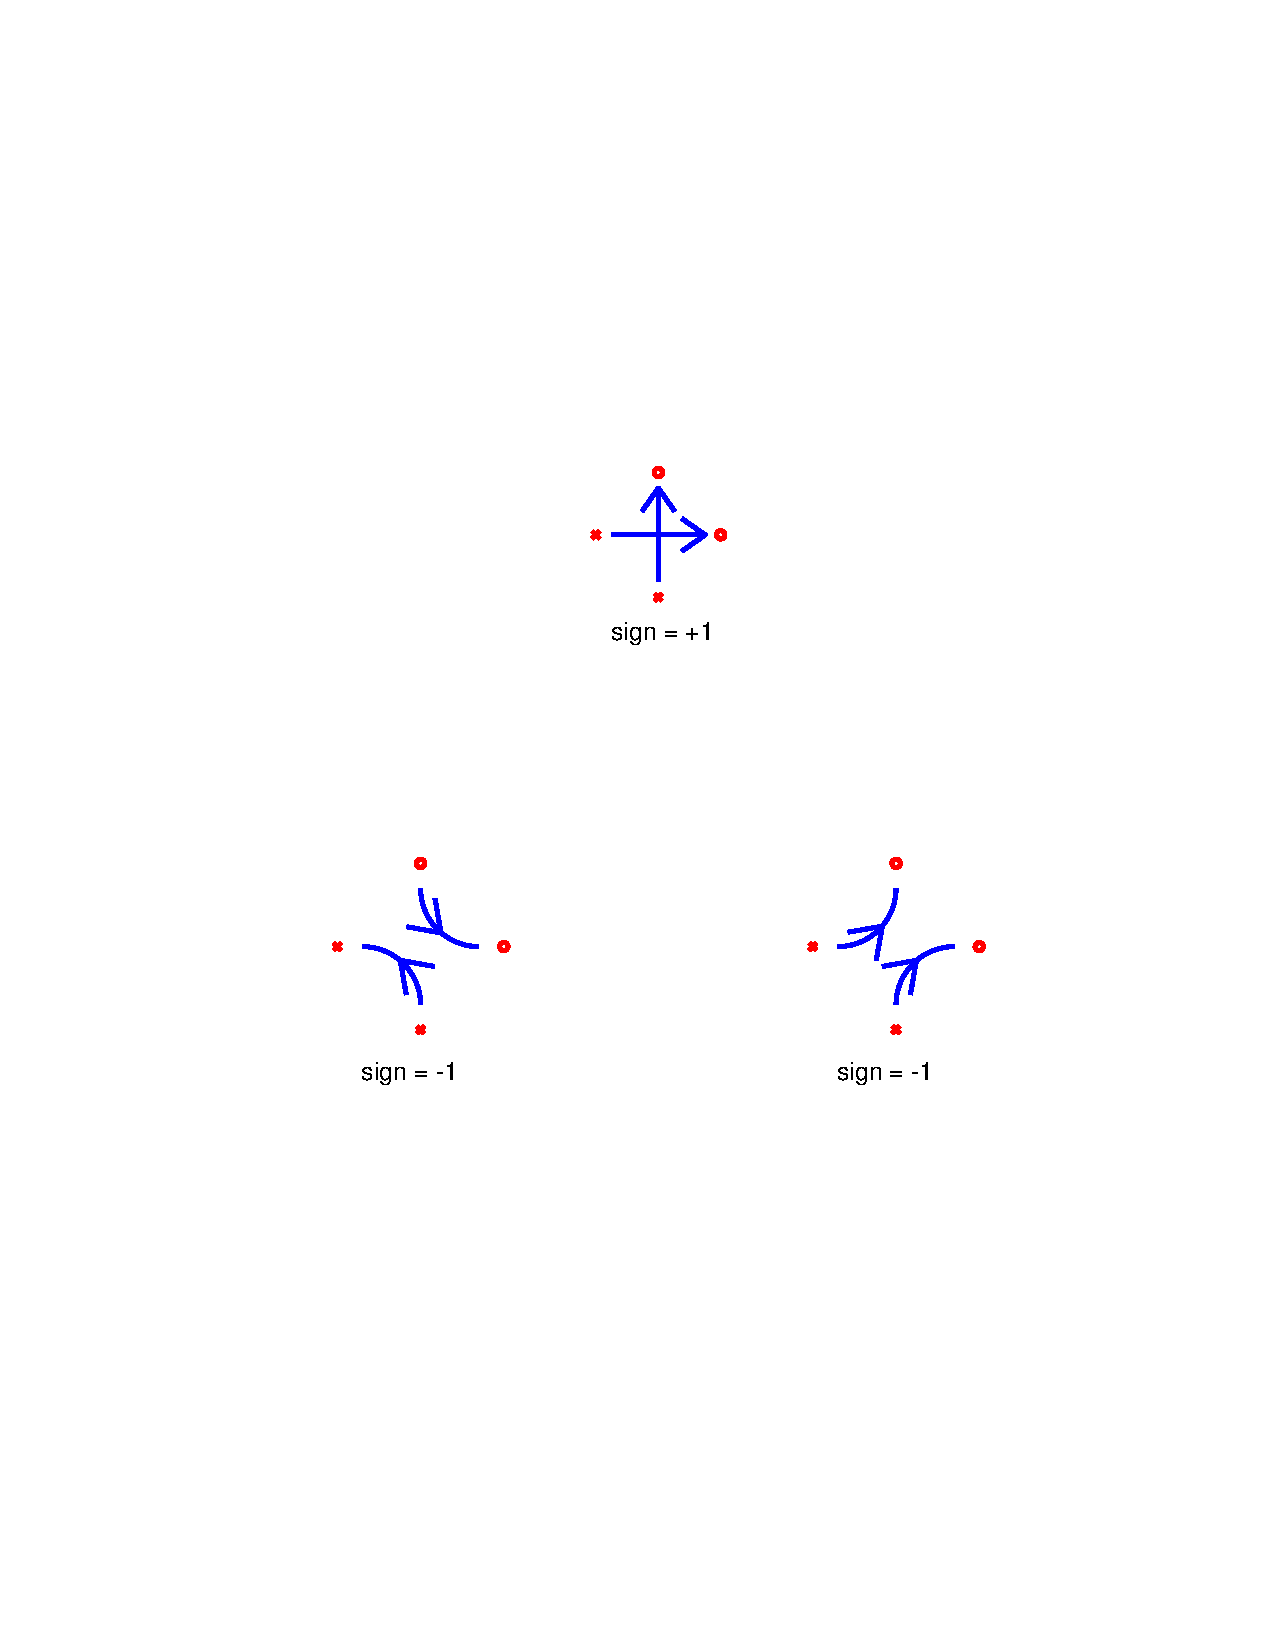
\includegraphics[width=7.5cm]{monomers}
\caption{\it There are three possible combinations of GV-pairs that represent empty sites.
The weights add up to $-1$.\label{fig:empty_sites}}
\end{center}
\end{figure}
%


Next we consider the contribution of a closed loop. It is produced by a suitable product
of GV-pairs 
%
\begin{align*}
\prod_{n=1}^{L}  P_{n}
%\eta_{i^{n}_{1}}^{\sigma^{n}_{1},\alpha^{n}_{1}}\eta_{i^{n}_{2}}^{\sigma^{n}_{2},\alpha^{n}_{2}}\;.
\end{align*}
%
each consisting of two GVs with a site and a type index.

We pick out one  of the bond pairs. It has site indices 
$i_{1}, i_{2}$ and type indices $\alpha_{1},\alpha_{2}$. Then from the remaining set of 
GV-pairs we take the one that contains  in one of its two GVs the site index $i_{2}$ and 
the complement of $\alpha_{2}$, i.e. $\overline \alpha_{2}$. By the complement we mean the opposite \mode value but the same directional value, i.e.
$(h x)\leftrightarrow (h o)$ and $(v x)\leftrightarrow (v o)$. The other variable shall have
site index $i_{3}$ and type index $\alpha_{3}$. 
If the first operator in the second GV-pair is the one that matches the second variable of the first pair, then we have a factor +1 otherwise a factor -1. 

When we use the graphical representation of the GV-pairs, the first is an arrow with an $x$
at its beginning and an $o$ at its end. Now we attache the graphical element of the second GV-pair. The arrow already indicates whether or not the variables are in the required order.
I.e. If we move opposite the arrow direction we get a minus sign. In addition, if the contracted
pair of variables $\eta_{i_{2}}^{\alpha_{2}}$ and $\eta_{i_{2}}^{\overline \alpha_{2}}$
have the \modes $ox$ that the trace gives +1 otherwise for $xo$ we obtain $-1$.
Next, we seek again the pair that now contains site
$i_{3}$ and type $\overline \alpha_{3}$.
Again we obtain a factor -1 if we move opposite the arrow direction and another -1 if the \mode-sequence is $xo$.
Now we move on like this. 
At the last step there is a final dangling (not contracted) variable with site index that has to be equal to $i_{1}$ and a type index equal to $\overline \alpha_{1}$. Otherwise,
the trace   over these the GV-pairs vanishes and they do not form an admitted graph.
By now we have reordered  the blocks of GV pairs (which causes no sign).
Again we obtain the two possible signs. Finally, we move the dangling variable to the front
of the GV-pair product, which gives an additional minus sign. Finally, we analyze the sign of the so-produce \mode sequence at the first variable pair.
%
The procedure is represented in figure \ref{fig:example}.
\begin{figure}[h]
\begin{center}
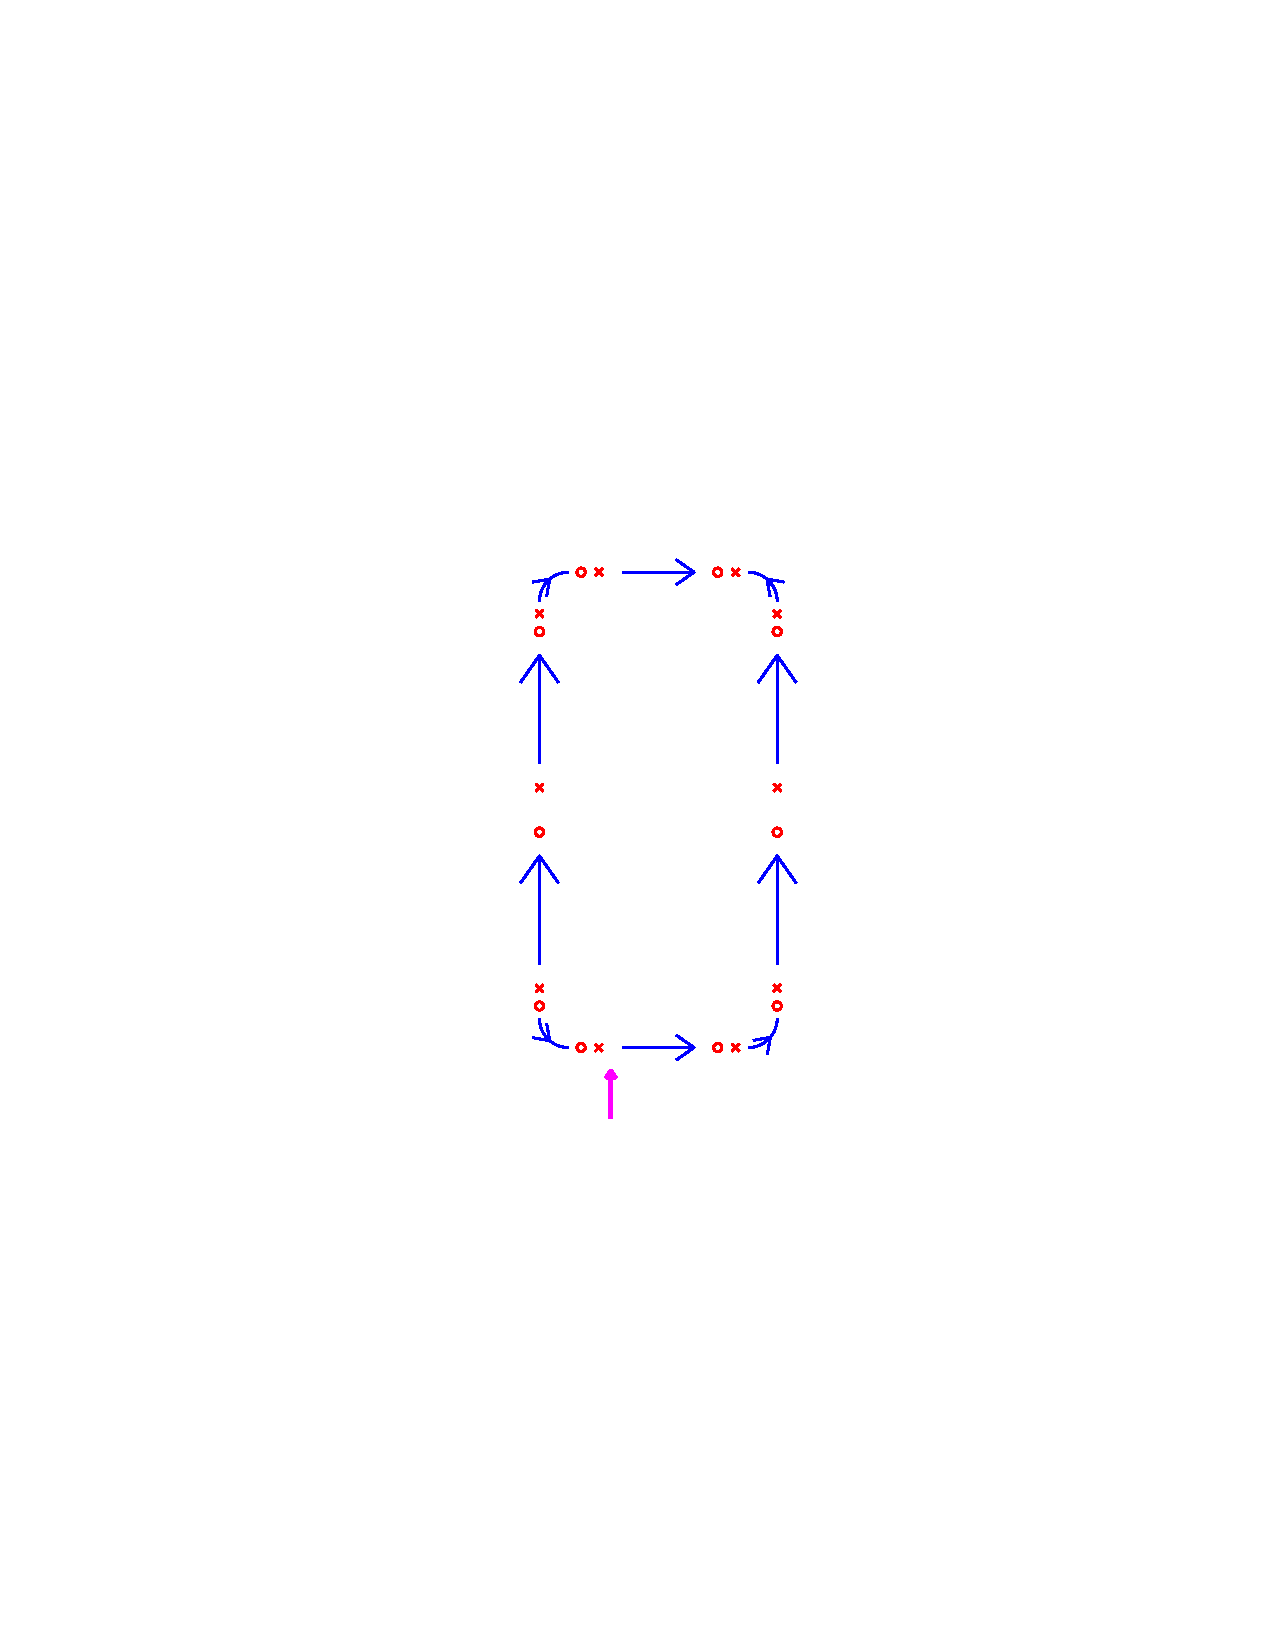
\includegraphics[width=7cm]{example}
\caption{{\it Example.\label{fig:example}}}
\end{center}
\end{figure}
%
We begin the tour with an  arrow of a graph-line, here the point indicated by the magenta arrow. 
Then we move to the right, the signs from the arrow directions are:
$+++++----+$, i.e. the sign of the arrows is $(-)^{4}=+1$. Next we count how often we have the \mode-sequence $xo$, when we move in the direction of the first arrow. There are 5 such 
events. Hence the sign factor is $(-1)^{5}=-1$. The two sign contributions give $-1$, together
with the additional -1 from moving the last variable to the front. The trace
of the product of GV-pairs is $+1$.


Keep in mind, that GV-pairs commute.


\clearpage 

\subsubsection{Basic elements of directed graphs}

In order to determine the weight of connected graph elements it is necessary to take
the direction into account, in which a graph is passed through. Therefore we have to consider directed graphs. Each graph has the  12 basic building blocks. There are 4 straight lines
as shown in figure \ref{fig:lines}, that go right, left, up, or down. 
%
\begin{figure}[h]
\begin{center}
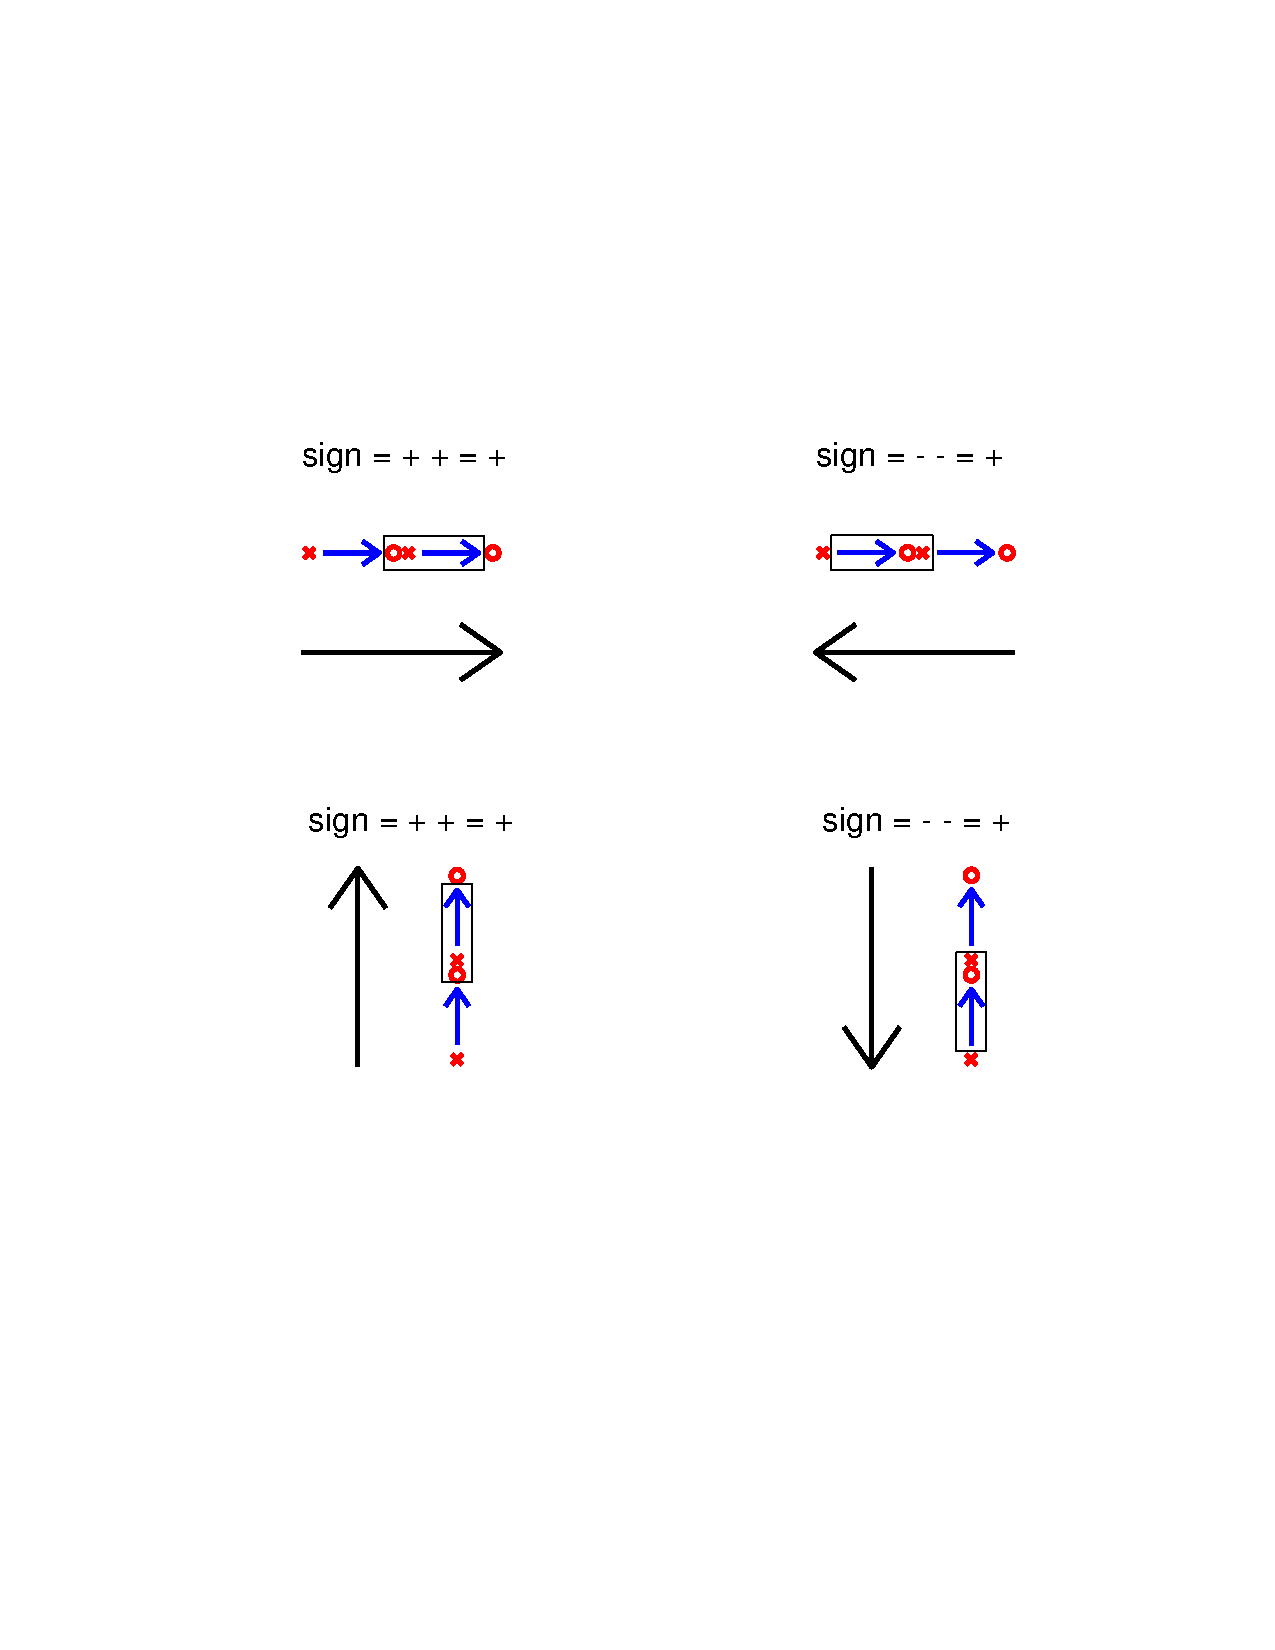
\includegraphics[width=8cm]{lines}
\caption{{\it The 4 different straight paths  and their signs. We see that they all have a positive sign.\label{fig:lines}}}
\end{center}
\end{figure}
%
The actual elements that form these lines are represented in the black boxes. In all cases the sign of the order of the \modes $ox$ and the arrow are the same, resulting in +1 for all 
lines. This is the sign that comes from the trace.

\clearpage
In addition to the lines  there are 8 different corners as depicted in 
figure \ref{fig:directed:graphs}
%
\begin{figure}[h]
\begin{center}
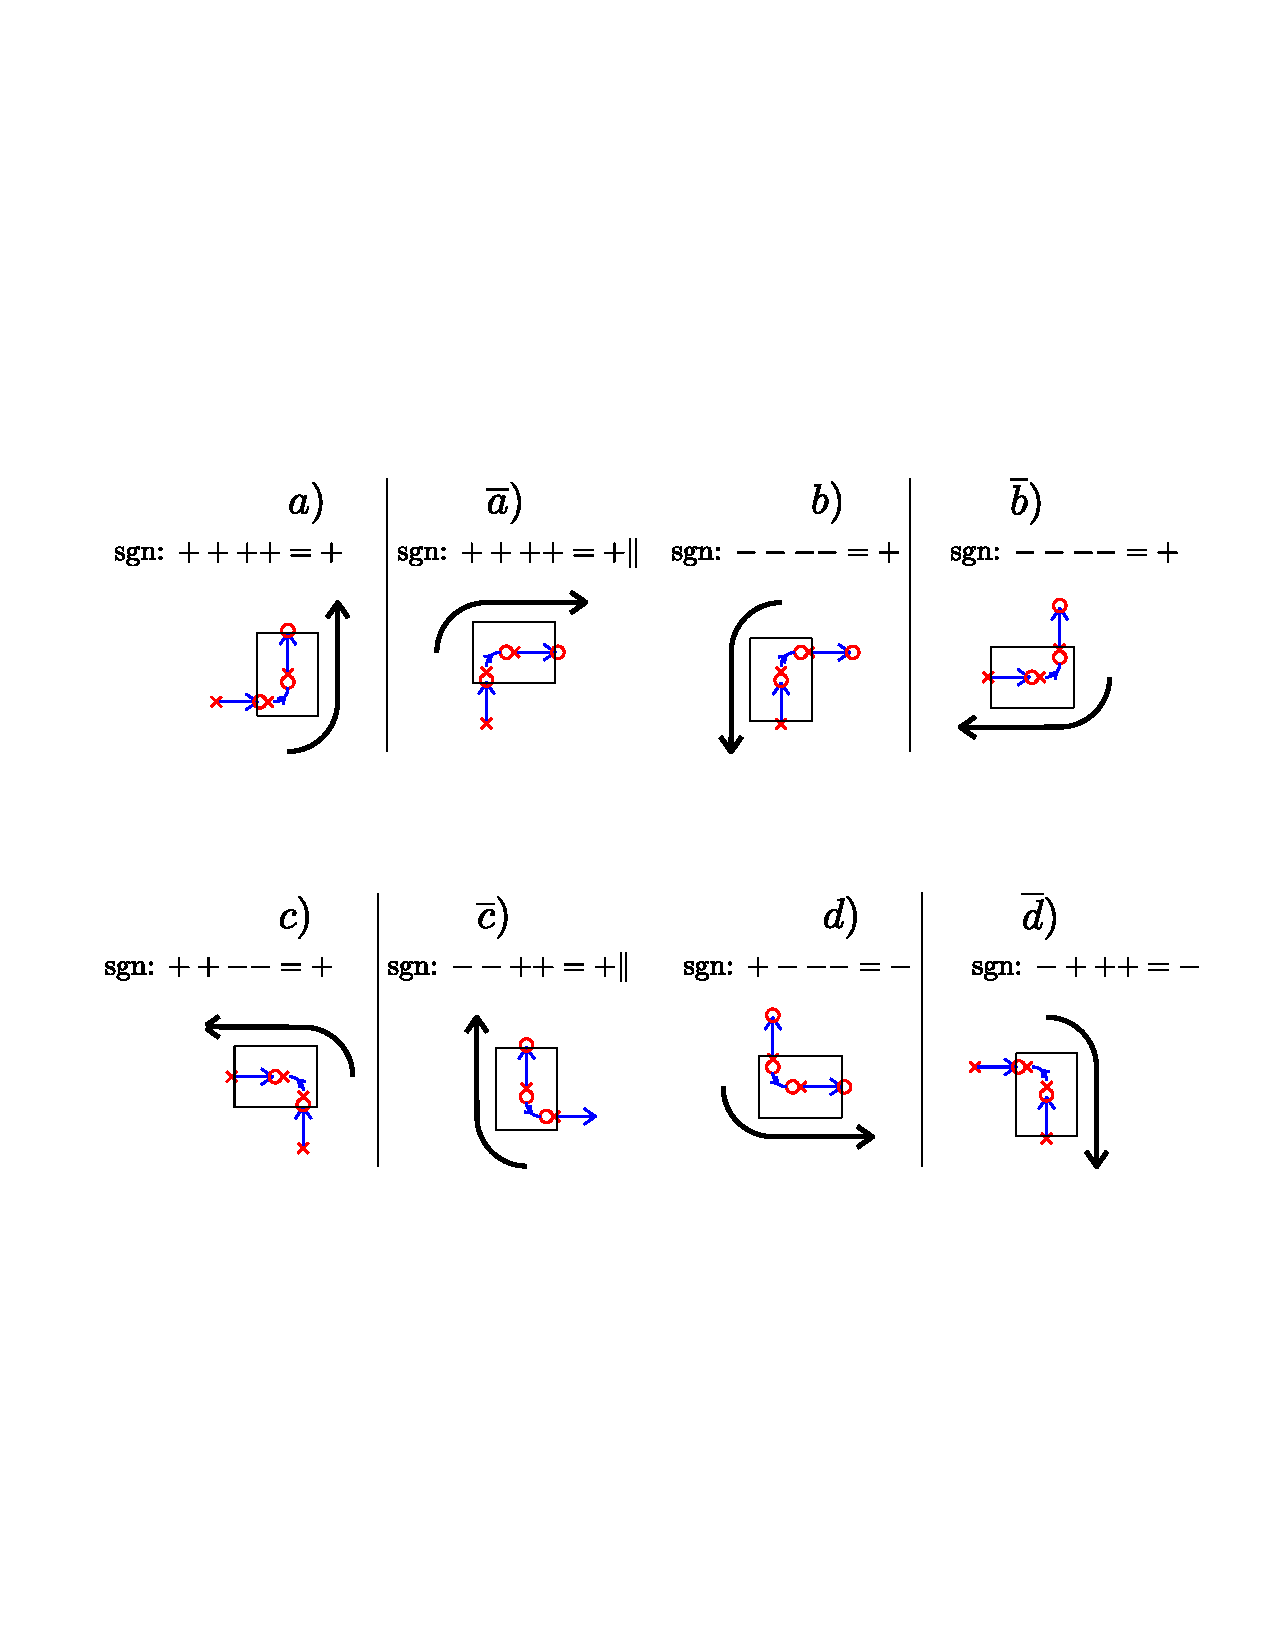
\includegraphics[width=12cm]{corners}
\caption{{\it The 8 different paths around a corner and their signs. The notation is chosen such, that paths $x$ and $\overline x$ start at end at the same connecting points to the rest of the graph, but they are bend in opposite directions.\label{fig:directed:graphs}}}
\end{center}
\end{figure}
%
With these elements we can construct any arbitrary graph  and compute the corresponding weight/ sign. Let us reconsider the example given in figure \ref{fig:example}.
\begin{figure}[h]
\begin{center}
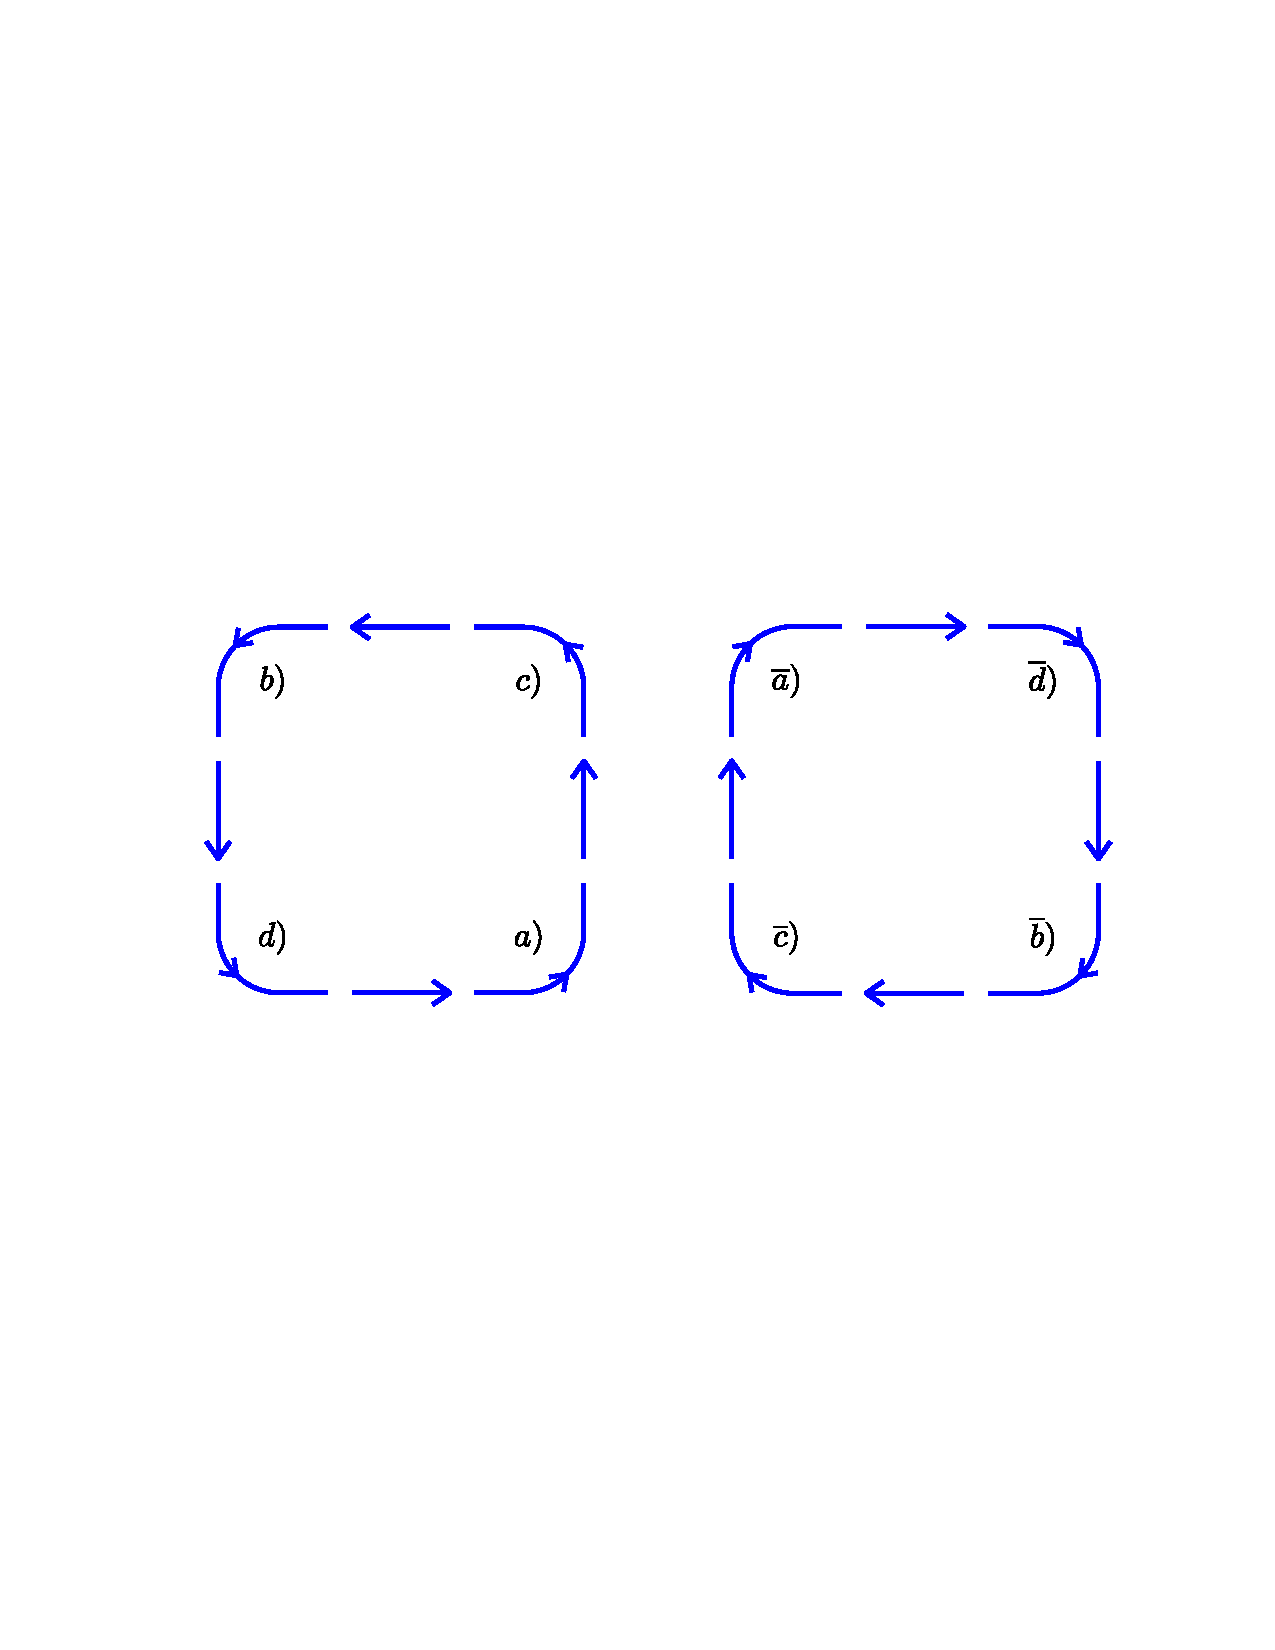
\includegraphics[width=6cm]{example_b}
\caption{{\it Example in directed graphs traversed in different directions.\label{fig:directed:graphs}}}
\end{center}
\end{figure}
%
We find the same sign as before, namely +1: we have one minus sign from corner $d$ or $\overline d$ and one sign from closing the loop. 
Lets now consider a more complex example of  closed non-overlapping loop:
%
\begin{figure}[h]
\begin{center}
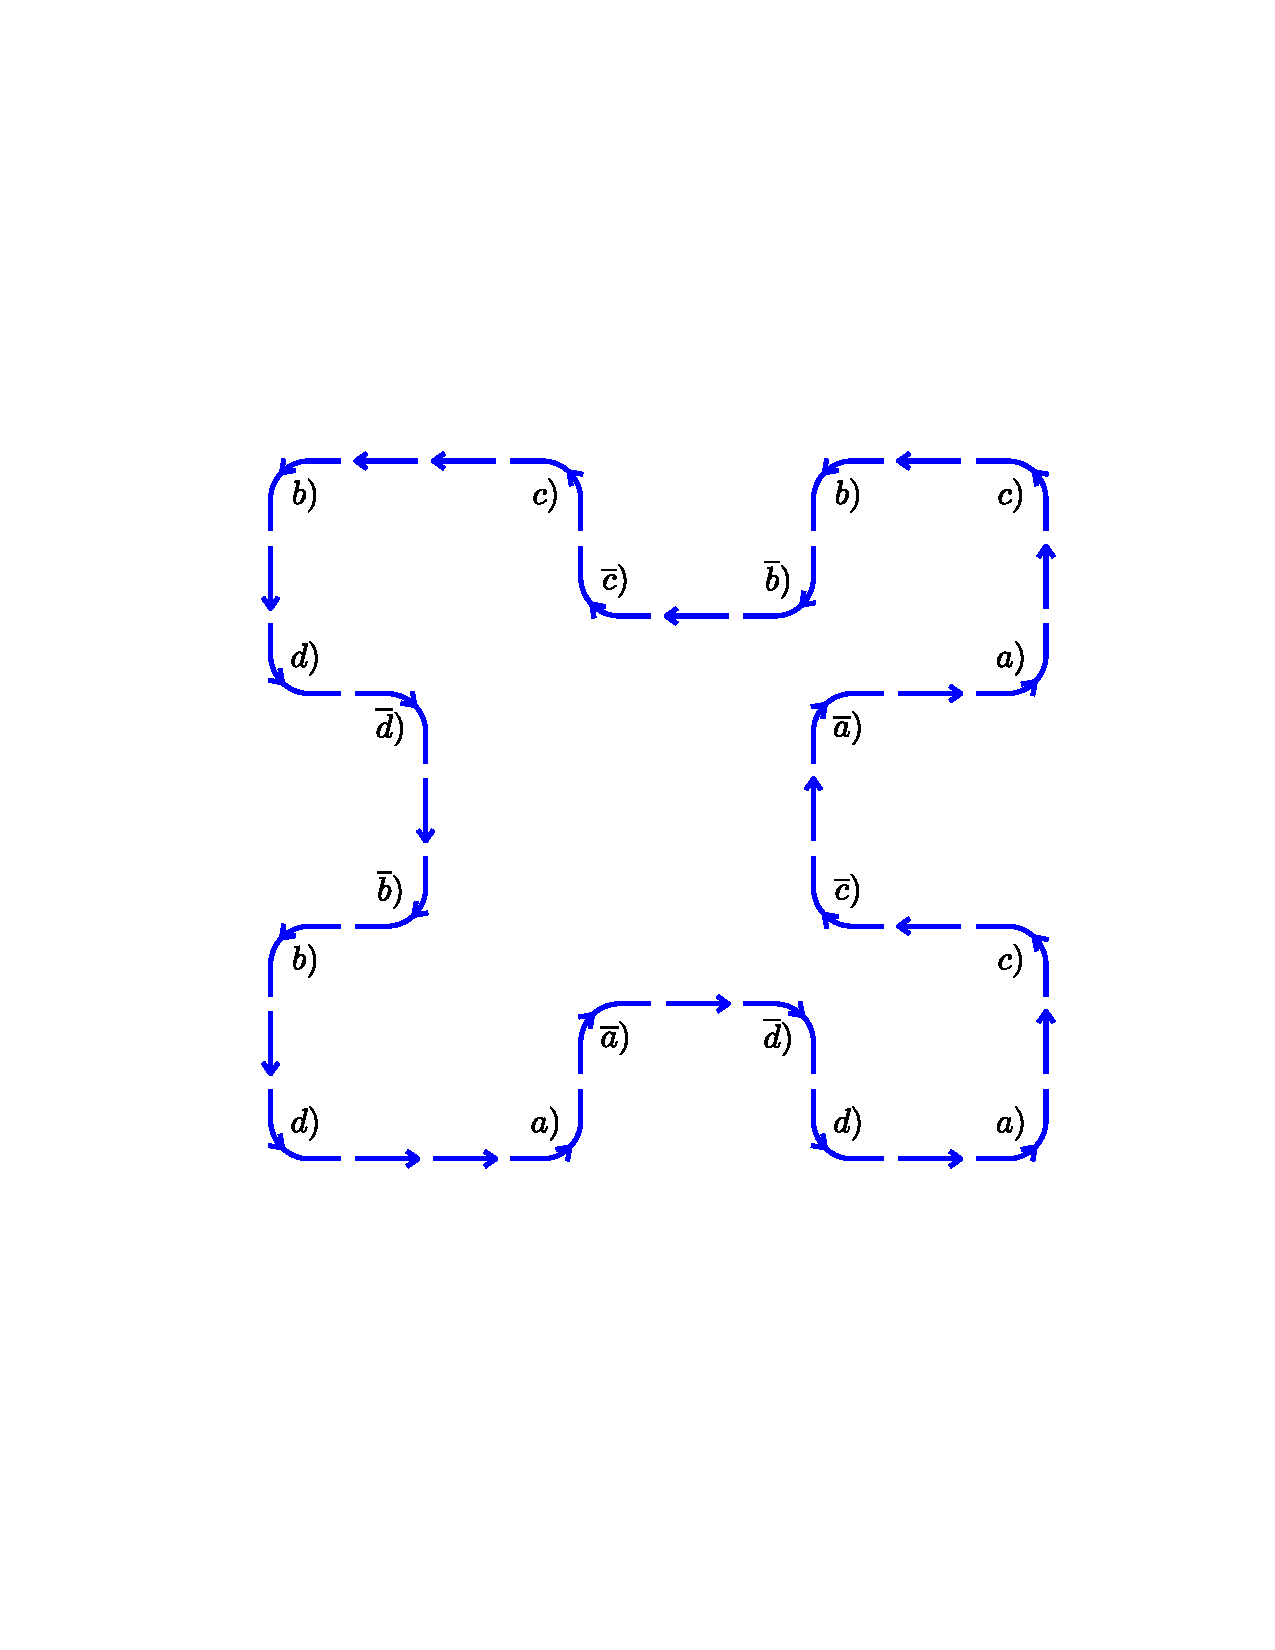
\includegraphics[width=10cm]{example_c}
\caption{{\it More complex example for directed graphs.\label{fig:directed:graphs_more}}}
\end{center}
\end{figure}
%

We can start any closed non-crossing loop  from the simple, square which has a positive sign, and then 
deform it. Each elementary deformation consists of  $x-\overline{x}$-pairs, as can be seen in 
figure \ref{fig:directed:graphs_more}. But the sign of such pairs is always one. Hence,
a closed loops has positive sign


\clearpage

\subsubsection{Impact of the minus sign in the action terms}

To each corner there is associated a minus sign from the action. And also each monomer
required between  lines  passing straight through a site there is also a minus sign. Remember
that the trace over the monomer variables of a sing GV-pair is one. I.e. at each site of a loop we have a minus. Empty sites also have a minus as discussed before. The signs of the action terms does not contribute, since always two terms enter and the sign squared is always on.

We will see  next that also a crossing will yield a minus sign. From the GV-elements we do not get a minus sign






\subsubsection{Sign of crossings}




We consider 2 closed loops, represented by the ellipses connected by a crossing. 
The overall sign is obtained by the signs of the elements in the ellipses, the sign of the crossing and the sign for closing this single connected graph. As before, also polygons with 
crossing are formed by a unique sequence of GV-pairs. And we obtain one extra sign from moving the dangling variable from the end to the beginning (closing sign).
The direction of the path is uniquely given by the arrows. The directions how the crossing is 
passed through, specifies two isolated ellipses. In any case, the directions of the corners
are always pairs of the form $x$ and $\overline x$. 
The total sign of the two separated graph elements (GE) consists of the sign from the elements of the the two 
GE, The sign of the $x$-$\overline x$ pair and two closing sign. 
Corner pairs $x$ / $\overline{x}$  both have the same starting and end point and are bend in opposite directions. On the other hand we know  the sign of the isolates objects already (proof by induction) as $S_{\text{l}_{i}}$. Then we have for the isolated loops
%
\begin{align*}
S_{\text{e}_{1}} * S_{\text{e}_{2}}  *
\underbrace{
S_{x} * S_{\overline x}
}_{\color{blue} = 1} * \underbrace{
S_{\text{closing}}^{2}
}_{\color{blue} = 1}
 &= S_{\text{l}_{1}} * S_{\text{l}_{2}}\\
\Rightarrow\qquad S_{\text{e}_{1}} * S_{\text{e}_{2}}
&= S_{\text{GE}_{1}} * S_{\text{GE}_{2}}\;.
\end{align*}
%
and the overall sign of the connected graph, that has  only one additional crossing is 
%
\begin{align}\label{eq:signrule:crossing}
S_{\text{total}} &= 
S_{\text{e}_{1}} * S_{\text{e}_{2}} * \underbrace{
S_{\text{str.lines}}
}_{\color{blue} = 1} * \underbrace{S_{\text{closing}}}_{\color{blue} = -1} = - S_{\text{GE}_{1}} * S_{\text{GE}_{2}}
\end{align}
%
Of course, the disconnected graph elements have to be shifted apart to obtain an admissible graph, but that has no impact on the sign argument.

Let's begin with a situation, where the separated graph elements are simple loops. Then both have a positive sign. The resulting connected graph with one crossing then has a negative sign.

%We are prompted to claim  that the sign of a connected graph element is $(-1)N_{c}$, where $N_{c}$ is the number of crossings.

We pick out any connected graph  elements with $N_{c}\ge 1$ and separat it at  one of the crossings, such that one of the  resulting separate objects is a loop with zero crossings and the other has therefore $N_{c}-1$ crossings. The sign of a graph element with $N_{c}$ crossings is then according \eq{eq:signrule:crossing}
%
\begin{align*}
S_{N_{c}} &= (-1) * S_{N_{c}-1} * \underbrace{
S_{N_{c}=0}
}_{\color{blue} = 1} = -S_{N_{c}-1}\\
\Rightarrow\qquad S_{N_{c}} &= (-1)^{N_{c}}\;.
\end{align*}
%
Hence each crossing in a graph introduces a minus sign. The origin is the trace. From the
building blocks there is no sign, as they are made of 4 bond GV-pairs, i.e.
they add a factor $t^{4}$, which is accounted for explicitly.

So we have the following situation: An empty site obtains a minus sign and  a site obtaining GV-pairs that from a crossing also have a minus sign, which results in both cases from the trace. The signs in front of the GV-s in the actions is +1 as the GV-pairs occur in pairs
in order to from an empty site or crossing.
This is different at straight lines and corners. At sites, where straight lines pass through,
a monomer is needed. Its contribution to the trace is +1, but it also has a weight factor
$a_{m}$, which now enters individually and not in pairs as in he case of empty sites. Hence
a site with a straight line passing through  gets a factor $a_{m}$. A site with a corner gets in addition to its contribution to the trace a factor $a_{c}$.

Since crossings and empty sites contribute unavoidably a minus sigh to the
corresponding sites, it is necessary to choose $a_{m}=a_{corner}=-1$, to make all sites equal.
Now they all contribute $-1$. Hence, we have to correct the partition function by an overall
factor 
%
\begin{align*}
(-1)^{N}\;,
\end{align*}
%
which in case of an even number of sites vanishes.



\subsection{Boundary Conditions}
We have fond so far that the sign of closed of all graphs is $(-1)^{N}$, i.e. each site contributes a
minus sign. There are several possibilities
\begin{enumerate}
	\item A corner gets a sign from the minus sign in the action for corners
	\item A straight line gets a sign from the minus sign from the corresponding monomer (which is perpendicular to the line)
	\item Empty sites have a minus sign as discussed before
	\item Crossings add a minus sign as discussed before.
\end{enumerate}
Wha we discussed so far is only  concerning the signs is only true for loops that do not close 
across a boundary.
Let's consider e.g. a straight horizontal line that is closed due to periodic boundary conditions across the boundary. Then we have schematically
%
\begin{align*}
&
\int \qty(\prod_{i} d\hdag{i} d\hnag{i})  \red{ \hdag{1}}\hnag{2}\hdag{2}\hnag{3} \cdots \hdag{N-1}\hnag{N}\hdag{N}\hnag{1} \\
&\qquad = 
- \int \qty(\prod_{i} d\hdag{i} d\hnag{i})   \hnag{2}\hdag{2}\hnag{3} \cdots \hdag{N-1}\hnag{N}\hdag{N}\hnag{1} \red{\hdag{1}}\\
&\qquad = 
-\prod_{i} \qty(\underbrace{
\int d\hdag{i} d\hnag{i} \; \hnag{i}\hdag{i}
}_{\color{blue} = 1})\\
&\qquad = - 1
\end{align*}
% 
In addition we have a minus sign on each site of the line from dangling monomer 
as discussed before. In comparison to a straight elements that are not part of a  closed loop across the boundary, there is an extra minus sign.

Unfortunately, the extra sign from the boundary is not simply given by the number of boundary crossings. That could be cured by aperiodic boundary conditions. 
Let's consider one horziontal and one vertical line closed across the boundary.
In that case both line are constructed by independent GV-pairs and the trace is merely the product of the individual traces, which gives $(-1)^{2}=+1$. In this situation, the crossing
does not give an extra minus sign, which it does when it is part of a graph that is not closed
across the boundary.

Hence, we cannot correctly count the graphs required for the Ising model with periodic boundary conditions by Grassmann variables and the action terms introduced so far.
For small $t$ values the impact of terms with winding number greater than one are unimportant, so we could use the Grassmann representation for small values of $t$ but not for the entire
interval $t\in(0,1)$. To avoid the sign problem we instead use open boundary conditions. Then
the graphs are all positively counted.



\subsection{Fourier transform of Grassmann variables} 
%todo Fourier transform GV
Although we are considering open boundary conditions, we still use the Fouriertrasnform
for periodic boundary conditions.
I.e., we  introduce the Fourier transform $\eta^{\alpha}_{\vv k}$ of the  GVs $\eta^{\alpha}_{i}$:
%
\begin{align}\label{eq:FT:GV}
 \eta^{\alpha}_{\vv k} &= \frac{1}{\sqrt{N}} \sum_{i}  \eta^{\alpha}_{i} e^{i \xx{i} \vv k}\\
  \eta^{\alpha}_{\xx{i}} &= \frac{1}{\sqrt{N}} \sum_{\vv k}^{1.b.z.}  \eta^{\alpha}_{\vv k} 
  e^{-i \xx{i} \vv k}\;,
\end{align}
%
with $k_{\alpha} = \frac{2\pi}{L_{\alpha}} n_{\alpha}$ with $n_{\alpha} = 0,1,\ldots L_{\alpha}-1$,
and for the integral
%
\begin{align}\label{eq:}
d \eta^{\alpha}_{\vv k} &= \frac{1}{\sqrt{N}} \sum_{i}  d\eta^{\alpha}_{i} e^{-i \xx{i} \vv k}\\
d  \eta^{\alpha}_{\xx{i}} &= \frac{1}{\sqrt{N}} \sum_{\vv k}^{1.b.z.}  d\eta^{\alpha}_{\vv k} 
  e^{i\xx{i} \vv k}\;.
\end{align}

The Fourier-transformed GVs are also GVs:
%
\begin{align}
 \eta^{\alpha}_{\vv k}  \eta^{\alpha'}_{\vv k'} 
 &= - \eta^{\alpha'}_{\vv k'}  \eta^{\alpha}_{\vv k}  \;,
\end{align}
%
which is seen by inserting the definition and using the anti-commuting properties of the
original GVs.
The FT GVs also have the correct integral properties, that follow from
%

\begin{subequations}
\begin{align}
\int d  \eta^{\alpha}_{\xx{i}} &= 0\label{eq:GV:int:a}\\
\int d  \eta^{\alpha}_{\xx{i}}\eta^{\alpha'}_{\xx{i'}} &= \delta_{\alpha\alpha'}\delta_{ii'}\;.
\label{eq:GV:int:b}
\end{align}
\end{subequations}

%
Then
%
\begin{align*}
\int d  \eta^{\alpha}_{\vv k} &= 0\\
\int d  \eta^{\alpha}_{\vv k} \eta^{\alpha'}_{\vv k'}&= \delta_{\vv k,\vv k'}\delta_{\alpha\alpha'} \;.
\end{align*}
%
The proof of the first property is simply obtained by inserting the definition of the 
FT and using \eq{eq:GV:int:a}. The proof of the second equation is as follows
%
\begin{align*}
\int d  \eta^{\alpha}_{\vv k} \eta^{\alpha'}_{\vv k'}
&=\frac{1}{N}\sum_{i,j} e^{i\big(-\vv k\xx{i} +\vv k'\xx{j}\big)} 
\underbrace{
\int d\eta^{\alpha}_{\xx{i}} \eta^{\alpha'}_{\xx{j}}
}_{\color{blue} = \delta_{i,j}\delta_{\alpha,\alpha'}}\\
&=\frac{1}{N}\sum_{i} e^{i\big(-\vv k +\vv k'\big)\xx{i}}   = \delta_{\vv k,\vv k'}
\end{align*}
%
The FT for the local action terms is simply 
\begin{subequations}\label{eq:}
\begin{align}
A_\text{corners} &=  -\sum_{\vv k} \big(\hdag{\vv k} \vnag{-\vv k}+\vdag{\vv k} \hnag{-\vv k}
+\vdag{\vv k} \hdag{-\vv k} +\vnag{\vv k} \hnag{-\vv k} \big)\\
A_\text{monomers} &=  \sum_{\vv k} \big(\hdag{\vv k} \hnag{-\vv k}
+\vdag{\vv k}\vnag{-\vv k} \big) \;.
\end{align}
\end{subequations}
%
The obc enters in the bond term.
For the treatment of the boundary condition it is best to introduce the  indices for the two directions
%
\begin{align*}
 A^{obc}_\text{bonds}  &= t \sum_{i=1}^{L_{x}-1} \sum_{j=1}^{L_{y}}
 \hdag{i,j} \hnag{i+1,j}
+ t \sum_{i=1}^{L_{x}} \sum_{j=1}^{L_{y}-1} \vdag{i,j} \vnag{i,j+1}\\
&= A^{pbc}  + \Delta A_\text{bonds}\\
\Delta A_\text{bonds} &=- \qty(t  \sum_{j=1}^{L_{y}}
 \hdag{N,j} \hnag{1,j}
+ t \sum_{i=1}^{L_{x}}\vdag{i,N} \vnag{i,1})\;.
\end{align*}
%
Then 
%
\begin{align*}
A^{pbc}_\text{bonds} &= \sum_{\vv k} \big(\varepsilon(k_{x}) \hdag{\vv k} \hnag{-\vv k}
+ \varepsilon(k_{y}) \vdag{\vv k} \vnag{-\vv k}\big)\\
\end{align*}
%
and
%
\begin{align*}
\Delta  A_\text{bonds}  
&=-\frac{t }{L_{x}L_{y}}\sum_{\vv k \vv k'} \hdag{\vv k}\hnag{\vv k'} 
\qty(\underbrace{
e^{- i \qty(k_{x} N + k'_{x} 1)}
}_{\color{blue} = e^{- i k'_{x}}}
\underbrace{
\sum_{j=1}^{L_{y}} e^{-i \qty(k_{y} j +  k'_{y} j)}
}_{\color{blue} = L_{y}\delta_{k'_{y},-k_{y}}})
\\
&\ldots- 
\frac{t }{L_{x}L_{y}}\sum_{\vv k \vv k'} \hdag{\vv k}\hnag{\vv k'} 
\qty(\underbrace{
e^{- i \qty(k_{y} N + k'_{y} 1)}
}_{\color{blue} = e^{- i k'_{y} }}
\underbrace{
\sum_{i=1}^{L_{x}} e^{-i \qty(k_{x} i +  k'_{x} i)}
}_{\color{blue} = L_{x} \delta_{k'_{x},-k_{x}}})\\
&=-\frac{t}{L_{x}} \sum_{k_{y}}\sum_{k_{x}k'_{x}} \hdag{ k_{x}k_{y}}\hnag{k'_{x},-k_{y}} 
e^{- i k'_{x}} -
\frac{t}{L_{y}} \sum_{k_{x}}\sum_{k_{y}k'_{y}}  \hdag{k_{x},k_{y}}\hnag{-k_{x},k'_{y}} 
e^{- i k'_{y} }
\end{align*}
%



 After FT the action reads
 %
\begin{subequations}\label{eq:}
\begin{align}
A &= A_\text{bonds}  + A_\text{corners}  + A_\text{monomers}\\
A_\text{bonds} &= \sum_{\vv k} \big(\varepsilon(k_{x}) \hdag{\vv k} \hnag{-\vv k}
+ \varepsilon(k_{y}) \vdag{\vv k} \vnag{-\vv k}\big)\\
A_\text{corners} &=  -\sum_{\vv k} \big(\hdag{\vv k} \vnag{-\vv k}+\vdag{\vv k} \hnag{-\vv k}
+\vdag{\vv k} \hdag{-\vv k} +\vnag{\vv k} \hnag{-\vv k} \big)\\
A_\text{monomers} &=  \sum_{\vv k} \big(\hdag{\vv k} \hnag{-\vv k}
+\vdag{\vv k}\vnag{-\vv k} \big) \;.
\end{align}
\end{subequations}
%
We can combine the bonds and the monomers to 

%
\begin{align*}
A_\text{bpm} &= \sum_{\vv k} \big(\tilde \varepsilon(k_{x}) \hdag{\vv k} \hnag{-\vv k}
+ \tilde \varepsilon(k_{y}) \vdag{\vv k} \vnag{-\vv k}\big)\\
\tilde \varepsilon(k) &= 1+\varepsilon(k)
=1 + t e^{i k} \;.
\end{align*}
%
In the sum we omit the term $\vv k=0$, as it has a vanishing contribution in the thermodynamic limit.
Next we use the ordering of the 
We can also use the GV-properties to symmetries the action by adding the term where the pair of GVs are swapped and $\vv k \to -\vv k$.
%
\begin{align*}
A &= A_\text{bpm}  + A_\text{corners}\\
A_\text{bpm} &=\frac{1}{2}\sum_{\vv k} \big(\tilde \varepsilon(k_{x}) \hdag{\vv k} \hnag{-\vv k}
-\tilde \varepsilon(-k_{x}) \hnag{\vv k} \hdag{-\vv k} 
+ \tilde \varepsilon(k_{y}) \vdag{\vv k} \vnag{-\vv k}
- \tilde \varepsilon(k_{y}) \vnag{\vv k} \vdag{-\vv k} 
\big)\\
A_\text{corners} &=  -\frac{1}{2}\sum_{\vv k} \big(
\hdag{\vv k} \vnag{-\vv k}
-\vnag{\vv k} \hdag{-\vv k} 
+\vdag{\vv k} \hnag{-\vv k}
- \hnag{\vv k}\vdag{-\vv k}\\
&\qquad\qquad     \ldots 
+\vdag{\vv k} \hdag{-\vv k} 
-\hdag{\vv k}  \vdag{-\vv k} 
+\vnag{\vv k} \hnag{-\vv k} 
- \hnag{\vv k} \vnag{-\vv k}\big)
\end{align*}
% 
We combine all GVs that belong to the same $\vv k$ into a vector.%
\begin{align*}
\vv \eta_{k} &= \big( \hdag{\vv k}, \hnag{\vv k}, \vdag{\vv k}, \vnag{\vv k}\big)^{T}
\end{align*}
%
Then the action can be written as
%
\begin{align*}
A &=  \frac{1}{2}\sum_{\vv k} \vv \eta_{\vv k}^{T}  M_{\vv k}  \eta_{-\vv k}
 =  \sum'_{\vv k} \vv \eta_{\vv k}^{T}  M_{\vv k}  \eta_{-\vv k}\;.\\
\text{with}\quad M_{\vv k} &=
\begin{pmatrix}
&h^{x}& h^{o}& v^{x} & v^{o}\\
\hline
h^{x}|&	0 & \tilde \varepsilon(k_{x}) & 1 & -1\\
h^{o}|&	-\tilde \varepsilon(-k_{x}) & 0  & 1 & 1\\
v^{x}|&	-1 & -1 & 0 & \tilde \varepsilon(k_{y})\\
v^{o}|&	1 & -1 & -\tilde \varepsilon(-k_{y}) & 0
\end{pmatrix}
\end{align*}
%
Here $M$ is an anti-Hermitian  matrix. The symbol $\sum'_{\vv k}$ indicates that $\vv k $ are only taken from the half plane $k_{y} > 0$ or $k_{y}=0$, if $k_{x > 0}$. The second half of the wave vectors is then given uniquely by $-\vv k$.
Moreover, the symbol $\sum'$
also excludes  $\vv k =0$, which has no impact in the thermodynamic limit. 

The Jakobi determinant of the transformation of the measure form real space to momentum space is +1, as outlined in appendix ??.

Then the vectors $\vv\eta_{\vv k} $
$\vv\eta_{-\vv k} $ contain independent GVs. Therefore, the trace gives
%
\begin{align*}
\tr{e^{A}} &= \prod'_{\vv k} \tr{e^{\sum_{\vv k} \vv \eta_{\vv k}^{T}  M_{\vv k}  \eta_{-\vv k}}}
=\prod_{\vv k}' \det\big( M_{\vv k} \big)\;.
\end{align*}
%
The determinant of $M_{\vv k}$ yields
%
\begin{align*}
\det\big( M_{\vv k} \big) &= \big( 1+t^{2} \big)^{2} - 2 t \big(1-t^{2}\big) \big( \cos(k_{x})
+\cos(k_{y}) \big)\;,
\end{align*}
%
which has the symmetry $\det\big( M_{-\vv k} \big) = \det\big( M_{\vv k} \big)$. So we can 
also include the second half plane in k-space in the product and also the term $\vv k=0$ as it 
has vanishing weight in the thermodynamic limit.
Finally, we have 

%
\begin{align}\label{eq:}
Z &= 2^{N} \cosh^{2N}(j) \prod_{\vv k}^{1.B.z.} \bigg( \big( 1+t^{2} \big)^{2} - 2 t \big(1-t^{2}\big) \big( \cos(k_{x})
+\cos(k_{y}) \big)\bigg)^{\frac{1}{2}}\;,
\end{align}
%
which is the Onsager result.


\section{Grassmann algebra}


An n-dimensional Grassmann algebra is the algebra generated by a set of (Grassmann) variables $\{\eta_{i}\}_{i=1:n}$,  satisfying
%
\begin{align}\label{eq:}
\{\eta_{i},\eta_{j}\}=0,  
\end{align}
%
i.e. they anti-commute, which implies in particular that $\eta_{i}^{2} = 0$. The algebra generated by these variables contains all expressions of the form
%
\begin{align*}
f(\eta) &= f_{0} + \sum_{i=1}^{n} f_{i} \eta_{i} + \sum_{i< j} f_{ij} \eta_{i} \eta_{j}
+\sum_{i< j<k} f_{ijk} \eta_{i} \eta_{j} \eta_{k} +\ldots + f_{1\ldots n}\; \eta_{1} \eta_{2} \ldots \eta_{n}\;. \;,
\end{align*}
%
with $f_{\bullet}\in \mathbb{C}$.
Obviously, the highest order term is 
%
\begin{align*}
f_{1\ldots n}\; \eta_{1} \eta_{2} \ldots \eta_{n}\;.
\end{align*}
%
since higher order terms would contain GVs in higher order which is zero.
%
We now define a left derivative $\partial_{i} := \partial_{a_{i}}$ . 
The derivative gives zero on a monomial which does not contain the variable $a_{i}$. 
If the monomial does contain $a_{i}$, it is moved to the left (with the appropriate sign due to the exchanges) and then suppressed. 
The operation is extended by linearity to any element of the algebra. 
A right derivative can be defined similarly. 
From this definition the following rules can be obtained
%
\begin{align*}
\{\partial_{a_{i}}, a_{j}\} &= \delta_{ij}\\
\{\partial_{a_{i}}, \partial_{a_{j}}\} &= 0\;.
\end{align*}
%
Integrals are defined as linear operations over the functions f with the property that they 
can be identified with the (left) derivatives. Correspondingly,
%
%
\begin{align}\label{eq:}
\int da_{i} f(a) &= \partial_{ a_{i}} f(a)\;.
\end{align}
%
Hence,
%
\begin{align*}
\int da_{i}  &= 0\\
\int da_{i} a_{j} &= \delta_{ij}\;.
\end{align*}
%
We also introduce a second set of GVs $\{\psi\}_{i=1:n}$ with the additional propetry
%
\begin{align*}
\{\psi_{i},\eta_{j}\} &= 0\;,\qquad \forall i,j\;.
\end{align*}
%
Next we compute exponentials of the form

%
\begin{align}\label{eq:gaussian:A}
\int\ldots\int \Dep e^{\vv\psi^{T} A \;\vv \eta} &=
\int\ldots\int \Dep\; e^{\frac{1}{2} \sum_{ij} \psi_{i} A_{ij} \eta_{j}}\\
&=\int\ldots\int \Dep \;\prod_{i<j} e^{A_{ij} \eta_{i}\eta_{j} }\\
&=\int\ldots\int \Dep \;\prod_{i<j} \underbrace{
\big(1 + A_{ij} \eta_{i}\eta_{j}\big)
}_{\color{blue} = B_{ij}}\;.
\end{align}
%
The Grassmann-measure is defined as
%
\begin{align*}
\Dep &:= \prod_{i} d \eta_{i} d\psi_{i}\;.
\end{align*}
%
Hence
%
\begin{align}\label{eq:fundamental:integral}
\int\ldots\int \Dep \prod_{i} \psi_{i} \eta_{i}&= 1\;.
\end{align}
%

We continue with \eq{eq:gaussian:A}
The double product can be formally written as
%
\begin{align}\label{eq:square:bracket}
\prod_{ij} B_{ij} &= \bigg[B_{11}\ldots B_{1n}\bigg]\times  \bigg[B_{21}\ldots B_{2n} \bigg]\times \ldots \times 
\bigg[ B_{n1}\ldots B_{nn}\bigg]
\end{align}
%
There are $2^{n^{2}}$ possible terms, by choosing  the 1 or the term $A_{ij}\psi_{i}\eta_{j}$ from each $B_{ij}$-term.
However, most of these combinations result in a vanishing trace because some of the GVs occur several times or not at all. The only choices that give a non vanishing contribution to the trace are as follows: From 
each  square bracket in \eq{eq:square:bracket}  choose one and only one $A_{i j} \psi_{i}\eta_{j}$ and the other terms contribute  1. 
The contribution of the $l$-th square brackets is
$A_{l,j_{l}} \psi_{l}\eta_{j_{l}}$.
Thus, each $\psi_{i}$ occurs precisely once. To ensure that this is also true for the $\eta_{j}$,
the set of indices  $\{j_{l}\}$ can only be permutations of the indices $\{1,2,\ldots,n\}$, which 
leads to
%
\begin{align}\label{eq:gaussian:B}
\int\ldots\int \Dep\; e^{\vv\psi^{T} A \;\vv \eta} &=
\sum_{\cP } \bigg(\prod_{l=1}^{n} A_{l,\cP _{l}}\bigg)\;\int\ldots\int \Dep 
\bigg( \prod_{l=l}^{n}\psi_{l} \eta_{\cP _{l}}  \bigg)\;.
\end{align}
%
Finally, we need to bring the permuted indices back into the natural order. To this end, we first
move the $\eta_{j}$ GVs to the very end, by retaining there mutual order, i.e.
\begin{align*}
\prod_{l}\psi_{l} \;\eta_{\cP _{l}}&= 
\text{sign} \cdot \prod_{l}\psi_{l} \;\prod_{l}\eta_{\cP _{l}}
\end{align*}
%
Here, $\text{sign}$ is the sign associated with separating the $\eta$- from the $\psi$-variables.
Next we bring the $\eta$-s into their natural order
\begin{align*}
\prod_{l}\psi_{l} \;\eta_{\cP _{l}}&= \text{sign} \big( \cP  \big)\cdot
\text{sign} \cdot \prod_{l}\psi_{l} \;\prod_{l}\eta_{l}
\end{align*}
%
Eventually, we form again the $\eta-\psi$-pairs, which again introduces the same sign as in the first step:
%
\begin{align*}
\prod_{l}\psi_{l} \;\eta_{\cP _{l}}&= \text{sign}\big( \cP  \big)
\big(\text{sign}\big)^{2} \prod_{l}\psi_{l} \eta_{l}\\
&=\text{sign}\big( \cP  \big)\prod_{l}\psi_{l} \eta_{l}
\end{align*}
%
Along with \eq{eq:fundamental:integral} and \eq{eq:gaussian:B}, we have
%
\begin{align*}
\int\ldots\int \Dep\; e^{\vv\psi^{T} A \;\vv \eta} &=
\sum_{\cP }\text{sign}\big( \cP  \big)\; \bigg(\prod_{l=1}^{n} A_{l,\cP _{l}}\bigg)\;.
\end{align*}
%
and finally
%
\tboxitp{Gaussian integral}{of type I}{
\begin{align}\label{eq:gaussian:C}
\int\ldots\int \Dep\; e^{\vv\psi^{T} A \;\vv \eta} 
&=\det\big( A \big)\;.
\end{align}}

\subsubsection{Gaussian integral II}




In this section we compute exponentials of the form
%
\begin{align}\label{eq:gaussian:II:A}
\int\ldots\int \Deta  e^{\frac{1}{2}\vv\eta^{T} A \;\vv \eta} &=
\int\ldots\int \Deta\; e^{\frac{1}{2}\sum_{ij} \eta_{i} A_{ij} \eta_{j}}\;.
\end{align}
%
The Grassmann-measure is defined now as
%
\begin{align*}
\Deta  &:= d \eta_{n} d \eta_{n-1} \ldots d \eta_{1}\;.
\end{align*}
%
In this case $A$ has to be anti-Hermitian/ skew-symmetric , i.e. 
%
\begin{align*}
A_{ji} &= - A_{ij}\\
\text{then}\quad \frac{1}{2}\sum_{ij} \eta_{i} A_{ij} \eta_{j} &=
\sum_{i<j} \eta_{i} A_{ij} \eta_{j}\;.
\end{align*}
%
We consider only the case of even dimension $n=2 m$.
Then
%
\begin{align}\label{eq:gaussian:II:B}
\int\ldots\int \Deta  e^{\frac{1}{2}\vv\eta^{T} A \;\vv \eta}
&=\int\ldots\int \Deta  \;\prod_{i<j} e^{A_{ij} \eta_{i}\eta_{j} }\\
&=\int\ldots\int \Deta \;\prod_{i<j} \underbrace{
\big(1 + A_{ij} \eta_{i}\eta_{j}\big)
}_{\color{blue} = B_{ij}}\\
\prod_{i<j} B_{ij} &= \bigg[B_{11}\ldots B_{1n}\bigg]\times  \bigg[B_{23}\ldots B_{2n} \bigg]\times \ldots \times \label{eq:Bs}
\end{align}
%
Each $B_{ij}$ contributes either $1$ of $\kappa_{ij}:=A_{ij}\eta_{i}\eta_{j}$. The product 
splits into a sum of $2^{n*n}$ terms $\{T_{i}\}_{i=1:n*n}$.
But a   a non-vanishing  trace is only obtained if each GV occurs precisely once.
This means that non vanishing terms $T_{i}$ contain  $(n/2=m)$ $\kappa_{ij}$-terms, with
no indices in common, or rather: each index from the list $\{1,2,\ldots,n\}$ occurs once.
The $\kappa_{ij}$ terms describe a pairing between indices $i$ and $j$, with $i<j$.
The non-vanishing combinations $\kappa_{ij}$ terms therefore describes a
partitioning of the set $\{1,2,\ldots,2m\}$ into pairs,
described by 
%
\begin{align*}
\kappa_{i_{1},j_{1}},\kappa_{i_{2},j_{2}},\ldots,\kappa_{i_{m},j_{m}}\;.
\end{align*}
%
Moreover, according to \eq{eq:Bs}, we have 
%
\begin{align*}
i_{l}&< j_{l}\\
i_{1}&<i_{2}<i_{3}\ldots\\
j_{1}&<j_{2}<j_{3}\ldots\,.
\end{align*}
%
Clearly, in the set of $T_{i}$-s all possible pairings occur once and only once. 
%
The set of all such pairings be denote by $P$. An element $\alpha\in P$ is characterised by
%
\begin{align*}
\alpha &= \{(i^{\alpha}_{1},j^{\alpha}_{1}),(i^{\alpha}_{2},j^{\alpha}_{2}),\ldots,(i^{\alpha}_{m},j^{\alpha}_{m})\}\;.
\end{align*}
%
$P$ has $(2m-1)!!$ elements. According to the construction for the non-vanishing trace elements,
we have $i^{\alpha}_{1}< i^{\alpha}_{2}<\ldots < i^{\alpha}_{m}$  and $i^{\alpha}_{l}< j^{\alpha}_{l}$. The contribution of such a partitioning to the trace is
%
\begin{align*}
\prod_{l} A_{i^{\alpha}_{l},j^{\alpha}_{l}} \cdot \int\ldots\int \Deta \;\prod_{l} \eta_{i^{\alpha}_{l}}\eta_{j^{\alpha}_{l}}\;.,
\end{align*}
%
Let $\cP (\alpha)$ be the permutation required to transform 
the sequence $i^{\alpha}_{1},j^{\alpha}_{1},i^{\alpha}_{2},j^{\alpha}_{2},\ldots,i^{\alpha}_{m},j^{\alpha}_{m}$ into the natural  sequence $1,2,\ldots,2m$ , then
%
\begin{align*}
\prod_{l} A_{i^{\alpha}_{l},j^{\alpha}_{l}} \cdot \int\ldots\int \Deta \;\prod_{l} \eta_{i^{\alpha}_{l}}\eta_{j^{\alpha}_{l}} &=\text{sign} (\cP (\alpha))\cdot 
\prod_{l} A_{i^{\alpha}_{l},j^{\alpha}_{l}}  \cdot \underbrace{
\int\ldots\int \Deta \;\prod_{i} \eta_{i}
}_{\color{blue} = 1}\;.
\end{align*}
%
Hence we have
\begin{align}\label{eq:gaussian:II:C}
\int\ldots\int \Deta  e^{\frac{1}{2}\vv\eta^{T} A \;\vv \eta}
&= \sum_{\alpha\in P}  
\text{sign} (\cP (\alpha))\;
\prod_{l=1}^{m} A_{i^{\alpha}_{l},j^{\alpha}_{l}} = \Pf{A})\;.
\end{align}
This is the definition of the Pfaffian. For $n=2m$ the Pfaffian is related to the determinant
via
%
\begin{align*}
\big(\Pf{A}\big)^{2} &= \det(A)
\end{align*}
%

For the proof we use
%
\begin{align*}
A &= U D U^{T}\\
D &=
\begin{pmatrix}
	0&\lambda_{1}&\ldots\\
	-\lambda_{1}&0&\ldots\\
	.&.&	0&\lambda_{2}&\ldots\\
	.&.&	-\lambda_{2}&0&\ldots\
\end{pmatrix}
\end{align*}
%
where $U$ is unitary. We use also
%
\begin{align}\label{eq:eta:xi}
\vv \eta = U \vv \xi\;,
\end{align}
%
and obtain
%
\begin{align*}
\frac{1}{2} \vv\eta^{T} A \vv \eta 
&= \frac{1}{2}\vv \xi^{T} D  \vv \xi\\
&= \sum_{\nu=1}^{m}  \lambda_{\nu} \xi_{2\nu-1}\xi_{2\nu}
\end{align*}
%
Then 
%
\begin{align*}
\int\ldots\int \Deta  e^{\frac{1}{2}\vv\eta^{T} A \;\vv \eta} 
&=\det\big( U \big) \int\ldots\int \Dxi   \prod_{\nu=1}^{m}
e^{\lambda_{\nu} \xi_{2\nu-1}\xi_{2\nu}} \\
&= \det\big( U \big)\prod_{\nu=1}^{m}  \int\int d \xi_{2\nu} d_{2\nu-1}
e^{\lambda_{\nu} \xi_{2\nu-1}\xi_{2\nu}} \\
&= \det\big( U \big)\prod_{\nu=1}^{m}  \underbrace{
\int\int d \xi_{2\nu} d_{2\nu-1}
\big(1+\lambda_{\nu} \xi_{2\nu-1}\xi_{2\nu}\big)
}_{\color{blue} = \lambda_{\nu}} \\
&= \det\big( U \big)\prod_{\nu=1}^{m} \lambda_{\nu} \;.
\end{align*}
%
Next we compute the determinant of $A$
%
\begin{align*}
\det\big( A \big) &=\det\big( U D U^{T} \big) =
\underbrace{
\big(\det(U)\big)^{2}
}_{\color{blue} = 1} \det(D)\\
&=
\det
\begin{pmatrix}
	0&\lambda_{1}&\ldots\\
	-\lambda_{1}&0&\ldots\\
	.&.&	0&\lambda_{2}&\ldots\\
	.&.&	-\lambda_{2}&0&\ldots\
\end{pmatrix}\\
&=
\prod_{\nu=1}^{m}
\det
\begin{pmatrix}
	0&\lambda_{\nu}\\
	-\lambda_{\nu}&0
\end{pmatrix}\\
&=\prod_{\nu=1}^{m} \lambda_{\nu}^{2}\\
&=\bigg(\prod_{\nu=1}^{m} \lambda_{\nu}\bigg)^{2}\\
&=\Pf{A}
\end{align*}
%


\subsubsection{Linear transformations}

We perform a linear transformation on a set of $n$ GVs $\{\eta\}_{i=1:n}$
%
\begin{align}
\eta_{i} &= A_{ij} \xi_{j};.
\end{align}
%
The anti commutator is
%
\begin{align*}
\{\eta_{i},\eta_{i'}\} &=A_{ij} A_{i'j'} \underbrace{
\{ \xi_{j},\xi_{j'}\} 
}_{\color{blue} = 0} = 0\;.
\end{align*}
%
For the differential  we need 
%
\begin{align*}
\partial_{\eta_{i}} \eta_{i'} &= \delta_{ii'}
\end{align*}
%
We expect that the differential $\partial_{\eta_{i}}$ will also be a linear function 
%
\begin{align*}
\partial_{\eta_{i}}ta &= B_{ij} \partial_{\xi_{j}}
\end{align*}
%
with the above constraint leading to
%
\begin{align*}
B_{ij}  A_{i'j'} 
\underbrace{
\partial_{\eta_{j}} \eta_{j'} 
}_{\color{blue} = \delta_{jj'}}
&= \delta_{ii'}\\
\big(B  A^{T} \big)_{ii'} &=  \delta_{ii'}\\
B A^{T} &= \uu\;.
\end{align*}
So we have
%
\begin{align}\label{eq:B:A}
B &= \big(A^{-1}\big)^{T}\;.
\end{align}
%
Especially for unitary transformations ($A^{-1}=A^{\dagger}$) we have
%
\begin{align*}
B &= \big(A^{\dagger}\big)^{T} = A^{*}\;.
\end{align*}
%

We are interested in these transformations in integrals
%
\begin{align*}
\int\ldots\int \Deta f(\eta)\;.
\end{align*}
%
Then
%
\begin{align*}
\Deta &= d \eta_{n} d\eta_{n-1} \ldots d\eta_{1} \\
&=- d \eta_{1} d\eta_{2} \ldots d\eta_{n} \\
&=-\sum_{\{l_{j}\}}\bigg(\prod_{j=1}^{n} B_{j l_{j}}\bigg) \; d \xi_{l_{1}}d \xi_{l_{2}}\ldots d \xi_{l_{n}}
\end{align*}
%
On the rhs each GV has to occur precisely once, otherwise there would be GVs that occur several times resulting in a vanishing contribution. Hence the sum over all indices is restricted to
a sum over all permutations ($\cP $) of the indices $1,\ldots,n$
%
\begin{align*}
\Deta 
%&= -\sum_{\{l_{j}\}}
%\bigg(\prod_{j=1}^{n} B_{j l_{j}}\bigg) \; d \xi_{l_{1}}d \xi_{l_{2}}\ldots d \xi_{l_{n}}\\
&=
-\sum_{\cP }
\bigg(\prod_{j=1}^{n} B_{j P_{j}}\bigg) \; d \xi_{P_{1}}d \xi_{P_{2}}\ldots d \xi_{P_{n}}\\
&=-
\underbrace{
\sum_{\cP }\text{sign}(\cP )\;
\bigg(\prod_{j=1}^{n} B_{j P_{j}}\bigg)
}_{\color{blue} = \det(B)} \; d \xi_{1}d \xi_{2}\ldots d \xi_{n}\\
&=\det(B) \; d \xi_{n}d \xi_{n-1}\ldots d \xi_{1}
\end{align*}
%
Hence the final result reads
%
\begin{align}\label{eq:}
\Deta &= \det(B) \;\Dxi 
\end{align}
%
Or rather along with \eq{eq:B:A} 
%
\begin{align}\label{eq:}
\int\ldots\int \Deta f(\eta) &= \det(A)^{-1}\; \int \ldots\int \Dxi \tilde f(\xi)\\
\tilde f(\xi) &= f(A\eta)\;.
\end{align}
%


	

Especially for the Fourier transformation we have
%
\begin{align*}
\eta_{j} &= \frac{1}{\sqrt{N}}\sum_{l} e^{i  \vv x_{j}\vv k_{l} } \xi_{l}\\
A_{j l} &= \frac{1}{\sqrt{N}} e^{i  x_{j}\vv k_{l}}\;.
\end{align*}
%
%
In the Ising application we have 4 different GVs at each site and we generalize the FT
accordingly
%
\begin{align}\label{eq:}
\eta^{\alpha}_{j} &= \frac{1}{\sqrt{N}}\sum_{l} e^{i  \vv x_{j}\vv k_{l} } \xi^{\alpha}_{l}\\
\end{align}
%
The measure was defined in \eq {eq:Disingi}. Here each variable $h^{x},h^{o},v^{x},v^{o}$ introduces a factor $\det(A)$. Since 
the Fourier transform is unitary, the determinant is $+/-$ and $\det^{4}(A) = 1$. We choose the order of $\vv k$-vectors as
%
\begin{align*}
\big(\vv 0\big),\big(\vv k_{1},-\vv k_{1}\big),\big(\vv k_{2},-\vv k_{2}\big),\ldots, \big(\vv k_{N/2},-\vv k_{N/2}\big)\;,
\end{align*}
% 
where the set $\vv k_{i}$ is chosen such that
%
\begin{align*}
k_{i,x} \le k_{i,y}\;.
\end{align*}
%

\section{Correlation functions}


We compute the correlation for an even number $2k$ of GVs. For odd the correlation is zero.
Proof: Let's start with one GV
%
\begin{align*}
\avg{\eta_{i}} &= \det(U) \sum_{l} U_{i,l}  \avg{\xi_{l}}\\
&=\det(U) \sum_{l} U_{i,l}  \Int \Dxi \xi_{l} \prod_{\nu=1}^{m} \bigg( 1 + \lambda_{\nu} 
\xi_{2\nu-1}\xi_{2\nu}\bigg)
\end{align*}
%
If $l=2\mu$

%
\begin{align*}
\avg{\eta_{i_{1}},\eta_{i_{2}},\ldots, \eta_{i_{2k}} } &=\frac{1}{Z}
\Int \Deta 
e^{\frac{1}{2}\vv \eta A \vv \eta}
\eta_{i_{1}},\eta_{i_{2}},\ldots, \eta_{i_{2k}}
\end{align*}
%
We use the transformation in \eq{eq:eta:xi} an obtain
\begin{align*}
\avg{\eta_{i_{1}},\eta_{i_{2}},\ldots, \eta_{i_{2k}} } &=\frac{1}{Z}
    \det(U)   
    \sum_{\{l_{i}\}} 
    \prod_{i=1}^{2 k} U_{i_{i},l_{i}}
    \Int \Deta 
    \prod_{\nu=1}^{m} e^{\lambda_{\nu} \xi_{2\nu-1}\xi_{2\nu}}\;
\xi_{l_{1}},\xi_{l_{2}},\ldots, \xi_{l_{2k}}
\end{align*}
Now a factor 
%
\begin{align*}
e^{\lambda_{\nu} \xi_{2\nu-1}\xi_{2\nu}} &=\bigg( 1+\lambda_{\nu} \xi_{2\nu-1}\xi_{2\nu}\bigg)
\end{align*}
%
ensures that from the pair of GVs  $\xi_{2\nu-1}\xi_{2\nu}$ either both variables occur (a) 
in the correlation factors or none (b). In case (b) the integral gives $\lambda_{\nu}$ and in case (a)the integral $\pm 1$. The sign depends on the position of the two GVs in the correlation-sequence. We recall that the partition function yield
%
\begin{align*}
Z &= \prod_{\nu=1}^{m} \lambda_{\nu}\;.
\end{align*}
%
The division by $Z$ therefore eliminates all factors $\lambda_{\nu}$ from the integrals of type $b$ and integrals of type
(a) are replaced by $\pm\lambda_{\nu}^{-1}$.

Hence, first we need  all complete (ordered, otherwise we would count twice) pairings $P$ of $2k$ elements and secondly we have to assign to each pair one of the possible index-pairs
%
\begin{align*}
\big(2\nu-1,2\nu\big)\;,
\end{align*}
%
or rather the index $\nu$.
Actually, none of the $\nu$-indices  should occur twice. On the other hand,
if they occur repeatedly,  the integral is zero anyways. Hence we allow the pairs to
have all indices $\nu=1,\ldots m$.
The sum over $\{l_{i}\}$ is replace by the sum over all elements $\alpha$ of complete (ordered) pairings, here represented by
$\{(i_{1}^{\alpha},i_{2}^{\alpha}),(i_{3}^{\alpha},i_{4}^{\alpha}),\ldots,(i_{2k-1}^{\alpha},i_{2k}^{\alpha})\}$, and all permutations  $\cP $ of these $2k$ indices. Hence
$l_{j}$ are replaced by $i^{\alpha}_{\cP _{j}}$.
Then we have
%
\begin{align*}
\avg{\eta_{i_{1}},\eta_{i_{2}},\ldots, \eta_{i_{2k}} } &=\frac{1}{Z}
    \det(U)  
    \prod_{i=1}^{2 k} U_{i_{i},l_{i}}
    \Int \Deta 
    \prod_{\nu=1}^{m} e^{\lambda_{\nu} \xi_{2\nu-1}\xi_{2\nu}}\;
\xi_{l_{1}},\xi_{l_{2}},\ldots, \xi_{l_{2k}}
\end{align*}


First we identify the pairing $\alpha\in P$ according to 
$\alpha=\{(I_{1}^{\alpha},J_{1}^{\alpha}),(I_{2}^{\alpha},J_{2}^{\alpha}),\ldots,(I_{k}^{\alpha},J_{k}^{\alpha})\}$ and group the terms accordingly
%
\begin{align*}
\avg{\eta_{i_{1}},\eta_{i_{2}},\ldots, \eta_{i_{2k}} } &=
\frac{1}{Z}
    \det(U)      \sum_{\{l_{i}\}} 
    \Int \Deta 
    \prod_{\nu=1}^{m} e^{\lambda_{\nu} \xi_{2\nu-1}\xi_{2\nu}}\;
    %
\prod_{\nu=1}^{k} U_{i_{I_{\nu}^{\alpha}},l_{I_{\nu}^{\alpha}} }
U_{i_{J_{\nu}^{\alpha}},l_{J_{\nu}^{\alpha}} }  
\text{sign}(p(\alpha))\prod_{\nu=1}^{k} \xi_{l_{I_{\nu}^{\alpha}} }\xi_{l_{J_{\nu}^{\alpha}} }\\
&=
\frac{1}{Z}\text{sign}(p(\alpha))
    \det(U)     
    \Int \Deta 
    \prod_{\nu=1}^{m} e^{\lambda_{\nu} \xi_{2\nu-1}\xi_{2\nu}}\;
    %
\prod_{\nu=1}^{k}\bigg( \sum_{l_{I_{\nu}^{\alpha}},l_{J_{\nu}^{\alpha}}} U_{i_{I_{\nu}^{\alpha}},l_{I_{\nu}^{\alpha}} }
U_{i_{J_{\nu}^{\alpha}},l_{J_{\nu}^{\alpha}} }   \xi_{l_{I_{\nu}^{\alpha}} }
\xi_{l_{J_{\nu}^{\alpha}} }\bigg)\;.
%
\end{align*}
%
The sign is necessary, since we have permuted the GVs such that pairs are nearest neighbours
and also have increasing indices in agreement with the definition of ordered pairings.
Now we can rename the summation indices 
%
\begin{align*}
\avg{\eta_{i_{1}},\eta_{i_{2}},\ldots, \eta_{i_{2k}} } 
&=
\frac{1}{Z}\text{sign}(p(\alpha))    \det(U)     \\
&\qquad \ldots
    \Int \Deta 
    \prod_{\nu=1}^{m} e^{\lambda_{\nu} \xi_{2\nu-1}\xi_{2\nu}}\;
    %
\prod_{\nu=1}^{k}\bigg( \sum_{l_1,l_{2}} U_{i_{I_{\nu}^{\alpha}},l_{1}}
U_{i_{J_{\nu}^{\alpha}},l_{2}}   \xi_{l_1}\xi_{l_2}\bigg)\;.
%
\end{align*}
%
The idea of the pairing was to identify two GVs that belong  to an index-pair of the form
$(2\nu-1,2\nu)$. Each pair should have a different index $\nu$. On the other hand, it does not matter if several pairs have the same index as the contribution is zero. 


So the indices
$(l_{1},l_{2})$ can run over all pairs of the form $(2\nu-1,2\nu)$, i.e.
%
\begin{align*}
\avg{\eta_{i_{1}},\eta_{i_{2}},\ldots, \eta_{i_{2k}} } 
&=
\frac{1}{Z}\text{sign}(p(\alpha))    \det(U)     \\
&\qquad \ldots
    \Int \Deta 
    \prod_{\nu=1}^{m} e^{\lambda_{\nu} \xi_{2\nu-1}\xi_{2\nu}}\;
    %
\prod_{\nu=1}^{k}\bigg( \sum_{\mu} U_{i_{I_{\nu}^{\alpha}},2\mu-1}
U_{i_{J_{\nu}^{\alpha}},2\mu}   \xi_{2\mu-1}\xi_{2\mu}\bigg)\;.
\end{align*}
%





\section{Correlations of type I}




For the Grassmann-pdf
%
\begin{align*}
e^{\vv \psi^{T} A \vv \eta} &=e^{\sum_{ij} \psi_{i} A_{ij}\eta_{j}}
\end{align*}
%
we compute the correlation function 
%
\begin{align*}
\avg{\psi_{i_{1}}\eta_{j_{1}}\psi_{i_{2}}\eta_{j_{2}}\ldots \psi_{i_{m}}\eta_{j_{m}}}\;.
\end{align*}
%
If the number of GVs of type $\psi$ and $\eta$ differ, the correlation is zero.
%
First we  introduce the index sets: 
%
\begin{align*}
I &=\{i_{1},i_{2},\ldots i_{m}\}\\
J &=\{j_{1},j_{2},\ldots j_{m}\}
\end{align*}
%
Next, we reorder the GVs such that the GVs in the correlator come first 
and the remaining GVs remain the original relative order.
%
\begin{align*}
\{\psi_{1}, \psi_{2}, \ldots \psi_{j_{m}}\}
&\longrightarrow 
\{\psi_{i_{1}}, \psi_{i_{2}}, \ldots \psi_{i_{m}},\ldots\}\\
\{\eta_{1}, \eta_{2}, \ldots \eta_{j_{m}}\}
&\longrightarrow 
\{\eta_{j_{1}}, \eta_{j_{2}}, \ldots \eta_{j_{m}},\ldots\}\\
\end{align*}
%
These reorderings can be achieved by permutations $\cP$ for the the GVs $\psi$
and $\cP'$ for the GVs $eta$. 
These reorderings of GVs are associated with  signs: $\sigma_{I}=\text{sign}(\cP)$
and $\sigma_{J}=\text{sign}(\cP')$, respectively.
As far as the measure $\Dep$ is concerned, we first separate the $\eta$
and $\psi$, resulting in some sign $\sigma$. Then we bring these terms into the new order, associated with the sign $\sigma_{I}\cdot \sigma_{J}$. Finally, we interleaf the $\eta$ and $\psi$ terms again. The last step
compensates the first sign $\sigma$. The new measure shall be denoted by 
$\Dept$, for which we have
%
\begin{align*}
\Dep &= \sigma_{I}\cdot \sigma_{J}\cdot\Dept\;.
\end{align*}
%
We continue with 
%
\begin{align*}
\avg{\psi_{j_{1}}\eta_{i_{1}}\psi_{j_{2}}\eta_{i_{2}}\ldots \psi_{j_{m}}\eta_{i_{m}}}
&=\frac{\sigma_{I}\; \sigma_{J}}{\det(A)}\;\Int \Dept  \; e^{\vv \psi^{T} A \vv \eta}\;
\psi_{i_{1}}\eta_{j_{1}}\psi_{i_{2}}\eta_{j_{2}}\ldots \psi_{i_{m}}\eta_{j_{m}}\\
&=\frac{\sigma_{I}\; \sigma_{J}}{\det(A)}\;\Int \Dept  \;\prod_{ij}\big( 1 + A_{ij} \psi_{i} \eta_{j}\big) \;
\psi_{i_{1}}\eta_{j_{1}}\psi_{i_{2}}\eta_{j_{2}}\ldots \psi_{i_{m}}\eta_{j_{m}}
\end{align*}
%
All terms $(1+A_{ij}\psi_{i}\eta_{j})$ with $i\in I$ or $j\in J$ can be replace by $1$, because
the  term $A_{ij} \psi_{i}\eta_{j}$ is multiplied $\psi_{i}$  or $\eta_{j}$, leading to GV$^{2}$. Then the integral  over the GVs contained in the
correlator terms can be performed ans gives $1$. Then we merely have to integrate over the remaining GVs 
%
\begin{align*}
\avg{\psi_{j_{1}}\eta_{i_{1}}\psi_{j_{2}}\eta_{i_{2}}\ldots \psi_{j_{m}}\eta_{i_{m}}}
&=\frac{\sigma_{I}\; \sigma_{J}}{\det(A)}\;\Int \Depx   \;
\bigg(\prod_{i\notin I, \;j\notin J}\big( 1 + A_{ij} \psi_{i} \eta_{j}\big)\bigg) 
\end{align*}
%
where $\Depx$ is the orignal measure $\Dep$ containing only  the indices 
$i\notin I$ and $j\notin J$.
The result is that of the partition function for the action matrix $A^{\canceledk{I}\canceledk{J}}$. Hence

%
\begin{align*}
\avg{\psi_{j_{1}}\eta_{i_{1}}\psi_{j_{2}}\eta_{i_{2}}\ldots \psi_{j_{m}}\eta_{i_{m}}}
&=\sigma_{I}\; \sigma_{J}
\;\frac{\det\big( A^{\canceledk{I}\canceledk{J}} \big)}{\det(A)}
\end{align*}
%
We recall that $A^{\canceledk{I}\canceledk{J}}$ is the matrix that is obtained by 
deleting the indices $I$ and $J$ in the rows and columns of $A$. 
To proceed, we reorder the indices of the matrix as we did above for the GVs, such that the indices in $I$ and $J$ come first. 
This is achieved by the permutation matrices (see section \ref{sec:permutation})
$P^{\cP}$ and $\cP'$.
We call the corresponding matrix $\hat   A$
%
\begin{align*}
\hat  A &= \big(P^{\cP}\big)^{T} A P^{\cP'}\;.
\end{align*}
%
Then for the determinant we have
%
\begin{align*}
\Det{\hat A} &= \Det{\big(P^{\cP}\big)^{T} A P^{\cP'}}\\
&=\Det{P^{\cP}} \Det{A} \Det{P^{\cP'}}\;.
\end{align*}
%
%
\begin{align*}
\Det{A}&=\Det{\hat A}\;\sigma_{I}\sigma_{J}
\end{align*}
%
We define the  block-structure of $\hat A$ as
%
\begin{align*}
\hat  A&= 
\begin{pmatrix}
\hat A_{11} &\hat A_{12}\\
\hat A_{2,1} & \hat A_{22}
\end{pmatrix}
=\begin{pmatrix}
 A^{IJ} & A^{I\canceledk{J}}\\
A^{\canceledk{I} J} &  A^{\canceledk{I}\canceledk{J}}\;.
\end{pmatrix}
\end{align*}
%
Where sub-block 11 contains $m\times m$ elements, namely those of the correlators. 
%
Then
%
\begin{align*}
\Det{A^{\canceledk{I}\canceledk{J}}}
&=\Det{\hat A_{22}}
\end{align*}
%
and therefore
\begin{align*}
\avg{\psi_{j_{1}}\eta_{i_{1}}\psi_{j_{2}}\eta_{i_{2}}\ldots \psi_{j_{m}}\eta_{i_{m}}}
&= \;\frac{\Det{ \hat A_{22} }}{\Det{\hat A}}
\end{align*}
%
According to \eq{eq:det:ratio} we have 
%
\begin{align*}
\avg{\psi_{j_{1}}\eta_{i_{1}}\psi_{j_{2}}\eta_{i_{2}}\ldots \psi_{j_{m}}\eta_{i_{m}}}&=
\Det{ \big(\hat A^{-1}\big)_{11}}
\end{align*}
%
and according to \eq{eq:inv:A:hat} we have
%
\begin{align*}
\hat A^{-1}&= \big(P^{\cP'}\big)^{T} A^{-1} P^{\cP}
\end{align*}
%
and hence
%
\begin{align*}
\avg{\psi_{j_{1}}\eta_{i_{1}}\psi_{j_{2}}\eta_{i_{2}}\ldots \psi_{j_{m}}\eta_{i_{m}}}
&=\Det{ \big(\big(P^{\cP'}\big)^{T} A^{-1} P^{\cP}\big)_{11}}\\
&=\Det{ \big(\big(A^{-1}\big)_{JI}}\;.
\end{align*}

Here $\big(A^{-1}\big)_{JI}$ is the sub matrix of the inverse of the original matrix $A$ taken at the indices $J$ and $I$.
%
A special case is
 \begin{align*}
\avg{\psi_{i}\eta_{j}}
&=\det\bigg( \big(A^{-1}\big)_{ji}\bigg)= \big(A^{-1}\big)_{ji}\;.
\end{align*}
%
Hence
%
\begin{align*}
\avg{\psi_{i_{1}}\eta_{j_{1}}\psi_{i_{2}}\eta_{j_{2}}\ldots \psi_{i_{m}}\eta_{j_{m}}}
&=\det\bigg(\avg{\psi_{I}\eta_{J}}\bigg)\;,
\end{align*}
%
which corresponds to the Wick expansion
%
\begin{align*}
\avg{\psi_{i_{1}}\eta_{j_{1}}\psi_{i_{2}}\eta_{j_{2}}\ldots \psi_{i_{m}}\eta_{j_{m}}}&=
\sum_{\cP } \sign{\cP } \prod_{l=1}^{m} \avg{\psi_{i_{l}} \eta_{j_{\cP _{l}}} }
\end{align*}
%




\section{Correlations of type II}




For the Grassmann-pdf
%
\begin{align*}
e^{\frac{1}{2}\vv \eta^{T} A \vv \eta} &=e^{\sum_{i<j} \eta_{i} A_{ij}\eta_{j}}
\end{align*}
%
where $A$ is antisymmetric, we compute the correlation function
%
\begin{align*}
\avg{\eta_{i_{1}}\eta_{i_{2}}\ldots \eta_{i_{2 m}}}\;.
\end{align*}
%
If the number of GVs has to be even, otherwise the correlation is zero.
%
First we  introduce the index set: 
%
\begin{align*}
I &=\{i_{1},i_{2},\ldots i_{2m}\}\;.
\end{align*}
%
We continue with 
%
\begin{align*}
\avg{\eta_{i_{1}}\eta_{i_{2}}\ldots \eta_{i_{2 m}}} 
&=\frac{1}{\text{Pf}(A)}\;\Int \Deta  \; e^{\frac{1}{2}\vv \eta^{T} A \vv \eta}\;
\eta_{i_{1}}\eta_{i_{2}}\ldots \eta_{i_{2 m}}\\
&=\frac{1}{\text{Pf}(A)}\;\Int \Deta  \; \prod_{i<j}
\bigg( 1 + a_{ij}\eta_{i}\eta_{j} \bigg)\;
\eta_{i_{1}}\eta_{i_{2}}\ldots \eta_{i_{2 m}}\;.
\end{align*}
%
All terms $(1+A_{ij}\eta_{i}\eta_{j})$ with $i\in I$ or $j\in I$ can be replace by $1$, because
the  term $A_{ij} \eta_{i}\eta_{j}$ is multiplied $\eta_{i}$  or $\eta_{j}$, leading to GV$^{2}$, which is zero. 


Next, we reorder the GVs such that the GVs in the correlator come first 
and the remaining GVs remain the original relative order.
%
\begin{align*}
\{\eta_{1}, \eta_{2}, \ldots \eta_{2m}\}
&\longrightarrow 
\{\eta_{i_{1}}, \eta_{i_{2}}, \ldots \eta_{i_{2m}},\ldots\}\;.
\end{align*}
%
This reordering of GVs are associated with a sign $\sigma_{I}$.
As far as the measure $\Deta$ is concerned, the reordering (here in reverse order) gives the same sign. 
The new measure shall be denoted by 
$\Detat$, and we have
%
\begin{align*}
\Deta  &= \sigma_{I}\;\Detat\;.
\end{align*}
%
Then the integral  over the GVs contained in the
correlator terms can be performed and it gives $1$. 


After that we only have to integrate over the remaining GVs 
%
%
\begin{align*}
\avg{\eta_{i_{1}}\eta_{i_{2}}\ldots \eta_{i_{2 m}}} 
&=\frac{\sigma_{I}}{\text{Pf}(A)}\;\Int \Detax  \; \prod_{i\notin I<j\notin I}
\bigg( 1 + a_{ij}\eta_{i}\eta_{j} \bigg)\;
\eta_{i_{1}}\eta_{i_{2}}\ldots \eta_{i_{2 m}}\;.
\end{align*}
%
%
where $\Detax$ is the orignal measure $\Deta$ containing only  the indices 
$i\notin I$.
The result is that of the partition function for the action matrix $A^{\canceledk{I}\canceledk{I}}$. 
Hence
%
\begin{align*}
\avg{\eta_{i_{1}}\eta_{i_{2}}\ldots \eta_{i_{2 m}}} 
&=\sigma_{I}\;
\;\frac{\Pf{ A^{\canceledk{I}\canceledk{I} } }}{\Pf{A}}
\end{align*}
%
We recall that $A^{\canceledk{I}\canceledk{I}}$ is the matrix that is obtained by 
deleting the indices $I$ in the rows and columns of $A$. 

For the next steps it is expedient, 
to introduce also the reordered matrix $A$, in which the indices contained in the correlator come first. Then
%
\begin{align*}
\hat A &= \big(P^{\cP}\big)^{T}  A P^{\cP}\;,
\end{align*}
%
with the block structure
%
\begin{align*}
\hat  A &= 
\begin{pmatrix}
\hat A_{11} &\hat A_{12}\\
\hat A_{21} & \hat  A_{22}
\end{pmatrix}
=
\begin{pmatrix}
A^{I,I} &A^{I,\canceledk{I}}\\
A^{\canceledk{I},I}& A^{\canceledk{I},\canceledk{I}}
\end{pmatrix}
\end{align*}
%
We use again
%
\begin{align*}
\Pf{\hat A} &= \Pf{P_{I}^{T}  A P_{I}}  = \Det{P_{I}} \Pf{A} = \sigma_{I} \Pf{A}\;.
\end{align*}
%
and
%
\begin{align*}
\Pf{A^{\canceledk{I}\canceledk{I}}}
&=\Pf{\hat A_{22}}\;,
\end{align*}
%
resulting in
\begin{align*}
\avg{\eta_{i_{1}}\eta_{i_{2}}\ldots\eta_{i_{m}}}
&=\frac{\Pf{ \hat A_{22}}}{\Pf{\hat A}}
\end{align*}

With \eq{eq:Pf:A:hat} we then have

\begin{align*}
\avg{\eta_{i_{1}}\eta_{i_{2}}\ldots\eta_{i_{m}}}
&=\Pf{ \big(- \hat A^{-1}\big)_{11}}
=\Pf{ \big(- A^{-1}\big)_{II}}
\end{align*}
Especially for $I=\{i_{1}i_{2}\}$ we obtain
\begin{align*}
\avg{\eta_{i_{1}}\eta_{i_{2}}}
=\Pf{ -
\begin{bmatrix}
0&\big(A^{-1}\big)_{i_{1}i_{2}}\\
-\big(A^{-1}\big)_{i_{1}i_{2}} & 0
\end{bmatrix}
} = - \big(A^{-1}\big)_{i_{1}i_{2}}
\end{align*}

So $\avg{\eta_{i_{1}}\eta_{i_{2}}}$ are the matrix elements of $-A^{-1}$ and 
we finally have
%
\begin{align}\label{eq:}
\avg{\eta_{i_{1}}\eta_{i_{2}}\ldots\eta_{i_{m}}} &=\Pf{M}
\intertext{where the $2m\times 2m$ matrix $M$ has the elements }
M_{ll'} &= \avg{\eta_{i_{l}}\eta_{i_{l'}}}
\end{align}
%
\section{Correlations in the Ising model}
%
For the spin-spin correlation we need
GV-correlations of the form
%
\begin{align*}
\avg{\prod_{l=1}^{m} \big(a + b\psi_{i_{l}} \eta_{j_{l}}\big)}
&= a^{m}\avg{\prod_{l=1}^{m} \big(1 + c\psi_{i_{l}} \eta_{j_{l}}\big)}
\end{align*}
%
with $c =b/a$. 
The correlator term can also be written as
%
%
\begin{align*}
\prod_{l=1}^{m} \big(1 + c\psi_{i_{l}} \eta_{j_{l}}\big) 
&=\prod_{l=1}^{m} e^{c\psi_{i_{l}} \eta_{j_{l}}} \\
&= e^{\sum_{l}c\psi_{i_{l}} \eta_{j_{l}}} \;.
\end{align*}
%
And
%
\begin{align*}
\sum_{l}c\psi_{i_{l}} \eta_{j_{l}}
&=
\sum_{l}c \qty(\sum_{i} \delta_{i,i_{l}} \psi_{i} )
\qty(\sum_{j} \delta_{j j_{l}} \eta_{j})\\
&= \sum_{ij} \underbrace{
\qty(\sum_{l} \delta_{i i_{l}} \delta_{j j_{l}})
}_{\color{blue} = C_{ij}} \Psi_{i}
\eta_{j}\;.
\end{align*}
%
We define the permutation matrices
%
\begin{align*}
\qty(P^{\cal P}) _{il} &= \delta_{i i_{l}}\\
\qty(P^{\cal P'} )_{ll} &= \delta_{j j_{l}}\;,
\end{align*}
%
The matrices $P^{\cP}$ and $P^{\cP'}$ have the size $N\times m$.
Then
%
\begin{align*}
C_{ij} &= \sum_{l} \delta_{i i_{l}} \delta_{j j_{l}} =\sum_{l}
\qty(P^{\cal P}) _{il} \qty(P^{\cal P'} )_{jl}
= \qty(P^{\cal P}  (P^{{\cal P}'})^{T} )_{ij}\\
\Rightarrow\qquad C &= P^{\cal P}  (P^{{\cal P}'})^{T} \;.
\end{align*}
%
Hence
%
\begin{align}\label{eq:}
\avg{\prod_{l=1}^{m} \big(1 + c\psi_{i_{l}} \eta_{j_{l}}\big)}
&=\frac{1}{\Det{A}} \Int \Dep 
e^{\vv \psi^{T} (A + C)\vv \eta}\\
&=\frac{\Det{A+C}}{\Det{A}}\\
&=\frac{\Det{A \big(\uu +A^{-1} C\big)}}{\Det{A}}\\
&=\frac{\Det{A}\Det{\uu +A^{-1} C}}{\Det{A}}\\
&=\Det{\uu +A^{-1} C}\;.
\end{align}
%
The Taylor expansion gives 
%
\begin{align*}
\ln\big(\Det{\uu +A^{-1} C}\big) &= \tr{\ln\big( \uu +A^{-1} C \big)}\\
&= \sum_{\nu=1}^{\infty} C_{\nu} c^{\nu} 
\tr{\big( A^{-1} P^{\cP} \big(P^{\cP'}\big)^{T}\big)^{\nu}}
\end{align*}
%
the trace terms are
%
\begin{align*}
\tr{\big( A^{-1} P^{\cP} \big(P^{\cP'}\big)^{T}\big)^{\nu}} &=
\tr{ A^{-1} \big(P^{\cP}\big)^{T}P^{\cP'} \ldots A^{-1} P^{\cP} \big( P^{\cP'}\big)^{T}}\\
&=\tr{ P^{\cP'} A^{-1} \big(P^{\cP}\big)^{T} P^{\cP'} \ldots A^{-1} \big(P^{\cP}\big)^{T}}\\
&=\tr{\bigg(\big(P^{\cP'}\big)^{T}   A^{-1} P^{\cP} \bigg)^{\nu}}
\end{align*}
%
Hence 
%
\begin{align*}
\Det{\uu_{N} + A^{-1}C} &= \Det{\uu_{m} + c \big(P^{\cP'}\big)^{T}   A^{-1} P^{\cP} }
\end{align*}
%
%
\begin{align*}
\bigg(\big(P^{\cP}\big)^{T}   A^{-1} P^{\cP'}\bigg)_{ll'} &=
\sum_{ji}P^{\cP'}_{j,l} \big(A^{-1}\big)_{ij}P^{\cP}_{il'}\\
&= \big(A^{-1}\big)_{j_{l}i_{l'}} \\
\big(P^{\cP}\big)^{T}   A^{-1} P^{\cP'} &= \big(A^{-1}\big)_{JI}
\end{align*}
%%
The correlation is therefore
%
\begin{align}\label{eq:}
\avg{\prod_{l=1}^{m} \big(a + b\psi_{i_{l}} \eta_{j_{l}}\big)}&=
a^{m}\avg{\prod_{l=1}^{m} \big(1 + c\psi_{i_{l}} \eta_{j_{l}}\big)}\\
&=a^{m} \Det{\big(\uu +c A^{-1}\big)_{JI}}\\
&= \Det{M}\\
M&= a \uu + b \big(A^{-1}\big)_{JI}\;.
\end{align}
%
For the simplest case we find
\begin{align}\label{eq:}
\avg{a + b\psi_{i} \eta_{j}} &=a + b\avg{\psi_{i} \eta_{j}} \\
\Rightarrow \big( A^{-1} \big)_{ji} &= \avg{\psi_{i} \eta_{j}} \;.
\end{align}
%
The final result therefore reads
%

\begin{subequations}\label{eq:GV:correlation}
\begin{align}
\avg{\prod_{l=1}^{m} \big(a + b\psi_{i_{l}} \eta_{j_{l}}\big)}&=\Det{M}\\
M_{ij} &= a \delta_{ij}  + \avg{\psi_{I_{i}} \eta_{J_{j}}}\;,
\qquad  i,j \in \{1,2,\ldots,m\}
\end{align}
\end{subequations}


\subsection{Transformation: spin correlation to  GV correlation}

We are interested in the spin-spin-correlation
%
\begin{align*}
C^{x}_{m}&:=\avg{\sigma_{\xx{0}}\sigma_{\xx{0} +m \vv e_{x}}}\;.
\end{align*}
%
Due to translational invariance, the result is independent of $\xx{0}$.
Since $\sigma_{i}^{2}=1$ we can replace the spin-spin-correlation function by
%
\begin{align*}
C^{x}_{m}&=\avg{\prod_{j=0}^{m-1}\sigma_{\xx{0} + j \vv e_{x}}\sigma_{\xx{0} + (j+1) \vv e_{x}}}\\
&=\avg{\prod_{\langle ij \rangle}^{\in L}\sigma_{\xx{i}} \sigma_{\xx{j}}} \;.
\end{align*}
%
where $\avg{i,j}$ are indices for nearest neighbour sites and $L$ is the set of such indices corresponding to the sites
of the form $\big(\xx{0} + j \vv e_{x}, \xx{0} + (j+1) \vv e_{x}\big)$, for $j=0,\ldots , m-1$.
Then
%
\begin{align*}
C^{x}_{m}
&=\frac{ch^{N}(\beta t)}{Z}\sum_{\{\sigma_{\xx{i}} \}}
\prod_{\langle ij \rangle} \bigg( 1+ t \sigma_{\xx{i}} \sigma_{\xx{j}} \bigg)
\prod_{\langle ij \rangle}^{\in L}\sigma_{\xx{i}} \sigma_{\xx{j}}\;.
\end{align*}
%

Next
%
\begin{align*}
\sum_{\{\sigma_{\xx{i}} \}}
\prod_{\langle ij \rangle} \bigg( 1+ t \sigma_{\xx{i}} \sigma_{\xx{j}} \bigg)
\prod_{\langle ij \rangle}^{\in L}\sigma_{\xx{i}} \sigma_{\xx{j}}
&=\sum_{\{\sigma_{\xx{i}} \}}
\prod_{\langle ij \rangle}^{\notin L} \bigg( 1+ t \sigma_{\xx{i}} \sigma_{\xx{j}} \bigg)
\prod_{\langle ij \rangle}^{\in L}\bigg[\bigg( 1+ t \sigma_{\xx{i}} \sigma_{\xx{j}} \bigg)\sigma_{\xx{i}} \sigma_{\xx{j}}\bigg]\\
&=\sum_{\{\sigma_{\xx{i}} \}}
\prod_{\langle ij \rangle}^{\notin L} \bigg( 1+ t \sigma_{\xx{i}} \sigma_{\xx{j}} \bigg)
\prod_{\langle ij \rangle}^{\in L}\bigg( \sigma_{\xx{i}} \sigma_{\xx{j}} + t \bigg)\\
&=\sum_{\{\sigma_{\xx{i}} \}}
\prod_{\langle ij \rangle}^{\notin L}\bigg( 1+ t \sigma_{\xx{i}} \sigma_{\xx{j}} \bigg)
\prod_{\langle ij \rangle}^{\in L}\bigg(1 + \frac{1}{t} \sigma_{\xx{i}} \sigma_{\xx{j}}  \bigg)\\
&=t^{m}\sum_{\{\sigma_{\xx{i}} \}}
\prod_{\langle ij \rangle}\bigg( 1+ \tilde t_{ij} \sigma_{\xx{i}} \sigma_{\xx{j}} \bigg)\;.
\end{align*}
%
with
%
\begin{align*}
\tilde t_{ij}&=
\begin{cases}
	t&\text{if }  ij\notin L\\
		t^{-1}&\text{if }  ij\in L
\end{cases}
\end{align*}
%
This is (apart from the prefactor) the partition function of an Ising model with modified
$t$. Then
%
\begin{align*}
C^{x}_{m} &= t^{m} \frac{Z(\tilde t\;)}{Z(t\;)}
= \frac{\tr{ e^{\tilde A}}}{\tr{ e^{A}}}\;.
\end{align*}
%
So it can be written as
%
\begin{align*}
\tr{ e^{\tilde A}}
&=\tr{ e^{A'} \prod_{ij}^{\in L}e^{t^{-1}\hdag{\xx{i}} \hnag{\xx{j}} }}   \\
\end{align*}
%
Here $A'$ is that part of the action, where the bonds on the nearest neighbour pairs
in $L$ are omitted.
%
\begin{align*}
t^{m}\tr{ e^{\tilde A}}
&=t^{m}\tr{ e^{A'} \prod_{ij}^{\in L}\;e^{t\hdag{\xx{i}} \hnag{\xx{j}} }
e^{-t\hdag{\xx{i}} \hnag{\xx{j}} } \; 
e^{t^{-1}\hdag{\xx{i}} \hnag{\xx{j}} }}\\
&=t^{m}\tr{ e^{A}\;
\prod_{ij}^{\in L}\;e^{(t^{-1}-t)\hdag{\xx{i}} \hnag{\xx{j}} }} \\
&=t^{m}\tr{ e^{A}\;
\prod_{ij}^{\in L}\;
\big(1 + (t^{-1}-t)\hdag{\xx{i}} \hnag{\xx{j}} \big)
} \;.
\end{align*}
%
Hence
%
\begin{align*}
C^{x}_{m} &= \frac{t^{m}\tr{ e^{\tilde A}}}{\tr{e^{A}}}\\
&=\frac{\tr{ e^{A}\;
\prod_{ij}^{\in L}\;
\big(t + (1-t^{2})\hdag{\xx{i}} \hnag{\xx{j}} \big)
}}{\tr{e^{A}}} \\
&=\avg{
\prod_{ij}^{\in L}\;
\big(t + (1-t^{2})\hdag{\xx{i}} \hnag{\xx{j}} \big)
} \;.
\end{align*}
%
In the present case for the spin-spin correlation in x-direction we have
\begin{align*}
C^{x}_{m} 
&=\avg{
\prod_{i=0}^{m-1}\;
\big(t + (1-t^{2})\hdag{(i,0)} \hnag{(i+1,0)} \big)
} \;.
\end{align*}
%
%
When we compare with \eq{eq:GV:correlation} the present case has
$I = \{(1,0),(2,0),\ldots(m,0)\}$
and $J=\{(2,0),(3,0),\ldots(m+1,0)\}$.
Hence
%
\begin{align}\label{eq:}
C^{x}_{m}&=\Det{M}\\
M_{ij} &= t \delta_{ij}  +(1-t^{2})
\avg{\hdag{I_{i}} \hnag{J_{j}}}\\
&= t \delta_{ij}  +(1-t^{2})
\avg{\hdag{i} \hnag{j+1}}\\
\end{align}
%

\subsection{Computation of pair-correlations}

We use translational invariance and the Fourier transformation defined in \eq{eq:FT:GV} and compute
%
\begin{align*}
\avg{\hdag{\xx{i}} \hnag{\xx{j}}}
&=\frac{1}{N}\sum_{l}\avg{\hdag{\xx{l}+\xx{i}} \hnag{  \xx{l} + \xx{j}}}\\ 
&=\frac{1}{N}\sum_{l}\;
\frac{1}{\sqrt{N}} \sum_{ \vv k}  e^{-i\vv k \big(\xx{l}+\xx{i}\big)}
\frac{1}{\sqrt{N}} \sum_{ \vv k'}
e^{-i \vv k' \big(\xx{l} +\xx{j}\big)}\;
\avg{\hdag{\vv k} \hnag{ \vv k'}}\\
&=\frac{1}{N}
\sum_{ \vv k, \vv k'}
\underbrace{
\bigg(\frac{1}{N}\sum_{l}\;
e^{-i \big(\vv k + \vv k'\big) \xx{l} }\bigg)
}_{\color{blue} = \delta_{\vv k', -\vv k}}\;
e^{-i\big(\vv k \xx{i} + \vv k' \xx{j}\big)}\;
\avg{\hdag{\vv k} \hnag{ \vv k'}}\\
%%%%
&=\frac{1}{N}
\sum_{ \vv k}
e^{i\big(\xx{j} -  \xx{i}\big)\vv k}\;
\avg{\hdag{\vv k} \hnag{- \vv k}}\;.
\end{align*}

Then 
%
\begin{align*}
\avg{\hdag{(i,0)} \hnag{(j+1,0)}} &=
\frac{1}{N}\sum_{ \vv k}
e^{i\big(j +1 -  i\big) k_{x}}\;
\avg{\hdag{\vv k} \hnag{- \vv k}}\;.
\end{align*}
%
and
%
\begin{align*}
\delta_{ij} &= 
\frac{1}{N}\sum_{ \vv k}
e^{i\big(j  -  i\big) k_{x}}\;.
\end{align*}
%
Therefore
%
\begin{align*}
M_{ij} &= \frac{1}{N}\sum_{ \vv k}
e^{i\big(j  -  i\big) k_{x}}
\bigg[ t + \big(1-t^{2}\big) e^{i k_{x}} \avg{\hdag{\vv k} \hnag{- \vv k}} \bigg]
\end{align*}
%
For the $\avg{\hdag{\vv k} \hnag{ -\vv k}}$ correlation we merely need to consider the subspace for this particular $\vv k$. The corresponding
action matrix is
%
\begin{align*}
A_{\vv k}&=
\begin{pmatrix}
&h^{x}& h^{o}& v^{x} & v^{o}\\
\hline
h^{x}|&	0 & \tilde \varepsilon(k_{x}) & 1 & -1\\
h^{o}|&	-\tilde \varepsilon(-k_{x}) & 0  & 1 & 1\\
v^{x}|&	-1 & -1 & 0 & \tilde \varepsilon(k_{y})\\
v^{o}|&	1 & -1 & -\tilde \varepsilon(-k_{y}) & 0
\end{pmatrix}
\end{align*}
%
In this enumeration we need 
%
\begin{align*}
\avg{\psi_{1}\eta_{2}} &=\big(A^{-1}\big)_{21}
\end{align*}
%%
We obtain with MATHEMATICA
\begin{align*}
\big(A_{\vv k}^{-1}\big)_{21} &= \frac{C_{\vv k}}{\Det{A_{\vv k}}}\\
C_{\vv k} &= - \big(\tilde \varepsilon(k_{y}) + \tilde \varepsilon(-k_{y})\big)
 +\tilde \varepsilon(-k_{x}) |\tilde \varepsilon(k_{y})|^{2} \\
\Det{A_{\vv k}} &= (1 + t^2)^2 - 2 t (1 - t^2) \big(\cos(k_{x})+\cos(k_{y})\big)\;.
\end{align*}
%




%todo current point
%
\section{Pfaffian}
\subsection{Definition}

Let $\Pi$ be the set of all partitions $\{1,2,\ldots,2n\}$ in pairs. 
Each element $\alpha\in \Pi$ can be be uniquely identified as 
%
\begin{align*}
\alpha &=\pairset{i}{j}{n}\;,
\end{align*}
%
it being understood that $\compset{i}{<}{n}$ and
$i_{k}<j_{k}\;\forall k$.
We define
%
\begin{align*}
\cP  &= 
\begin{bmatrix}
	1&2&3&4&\ldots& 2n-1&2n\\
	i_{1}&	j_{1} &	i_{2}	& j_{2} &\ldots &	i_{n} & j_{n}
\end{bmatrix}
\end{align*}
%
as the corresponding permutation and we define $\sign{\alpha} = \sign{\cP }$.

For any antisymmetric (skew-symmetric, alternating, i.e. $A_{ji}=-A_{iij}$) $2n\times 2n$ matrix $A$ the Pfaffian is defined as
%
\begin{align}\label{eq:}
\Pf{A} &=\sum_{\alpha\in \Pi} \sign{\alpha}\; \setprod{a}{i^{\alpha}}{j^{\alpha}}{n}\\
\Pf{A} &=\sum_{\alpha\in \Pi} \sign{\alpha}\; \Setprod{a}{i^{\alpha}}{j^{\alpha}}{n}
\end{align}
%

For anti-symmetric matrices of odd dimension the Pfaffian is defined as zero.


\subsection{Examples}

%
\begin{align*}
\Pf{
\begin{bmatrix}
	0&a\\-a&0
\end{bmatrix}
} &= a\\
%%%%%
\Pf{
\begin{bmatrix}
	0&\lambda_{1}&0&0\\
	-\lambda_{1}&0&\omega_{1}&0\\
	0&-\omega_{2}&0&\lambda_{2}\\
	0&0&-\lambda_{2}&0
\end{bmatrix}
} &= a_{12}a_{34} - a_{13}a_{24} + a_{14}a_{23}\\
&=\lambda_{1}\lambda_{2}\;.
\end{align*}
%

\subsection{Properties}
For any anti-symmetric $2n\times 2n$ matrix $A$ or $A_{l}$ and an arbitrary $2n\times 2n$ matrix $B$
holds 
%

\begin{subequations}\label{eq:}
\begin{align}
\qty(\Pf{A})^{2} &= \det(A)\\
\Pf{B A B^{T}} &= \det(B)\cdot \Pf{A}\\
\Pf{\lambda A} &= \lambda^{2}\Pf{A}\\
\Pf{A^{T}} &= (-1)^{n} \Pf{A}
\intertext{for block-diagonal matrices}
A = \oplus_{l=1}^{L} A_{l}
&=
\begin{pmatrix}
	A_{1}\\
	&\ddots\\
	&&A_{L}
\end{pmatrix}\nonumber\\
\text{holds}\; 
\Pf{A} &= \prod_{l=1}^{L} \Pf{A_{l}}
\intertext{for an arbitrary $n\times n$ matrix $M$ holds}
\Pf{
\begin{pmatrix}
	0&M\\
	-M^{T}&0
\end{pmatrix}
} &= (-1)^{\frac{n(n-1)}{2}}\;\det(M)\;.
\end{align}
\end{subequations}
%

The product of the Pfaffians of skew-symmetric matrices A and B \blue{under the condition that $A^{T}B$ is a positive-definite matrix} can be represented in the form of an exponential
%
\begin{align*}
{\displaystyle {\textrm {pf}}(A)\,{\textrm {pf}}(B)=\exp({\tfrac {1}{2}}\mathrm {tr} \log(A^{\text{T}}B)).}
\end{align*}
%
This is called the \blue{trace identity}.

Suppose $A$ is a $2n \times 2n$ skew-symmetric matrices, then
%
\begin{align*}
\textrm {pf}(A)=i^{(n^{2})}\exp \left({\tfrac {1}{2}}\mathrm {tr} \log((\sigma _{y}\otimes I_{n})^{T}\cdot A)\right)
\end{align*}
%,
where 
$\sigma_y$ is the second Pauli matrix
%
\begin{align*}
\sigma_{y} &= 
\mqty(0&-i\\i&0)\;,
\end{align*}
%
$I_{n}$ is an identity matrix of dimension $n$ and we took the trace over a matrix logarithm.
We have the block structure
%
\begin{align*}
\qty(\sigma_{y}\otimes I_{n})^{T} &=
\mqty(0& i I_{n}\\
-i I_{n}&0)
\end{align*}
%

This equality is based on the trace identity
and on the observation that 
%
\begin{align*}
\displaystyle {\textrm {pf}}(\sigma _{y}\otimes I_{n})
&=(-1)^{n(n-1)/2} \det(- i I_{n})\\
&=(-1)^{n(n-1)/2} (- i)^{n}\underbrace{
\det(I_{n})
}_{\color{blue} = }1\\
&=(-i)^{n^{2}}.
\end{align*}
%


\red{Is $(\sigma_{y}\otimes I_{n})^{T}$ really positiv}
Any anti-symmetric $2n\times 2n$ matrix $A$ can be written as
%
\begin{align*}
A &= U D U^{T}\;,
\end{align*}
%
where $U^{T}=U^{-1}$ with $\det(U) = 1$ \red{($det(U)=1$ can always be achieved by adjusting the sign of $\lambda_{\nu}$)} and
%
\begin{align*}
D &= \oplus_{\nu=1}^{n} D_{\nu}\\
D_{\nu} &= \begin{pmatrix}
	0 &\lambda_{\nu}\\
	-\lambda_{\nu}&0
\end{pmatrix}
\end{align*}
%
From that we can proof that
%
\begin{align*}
\Pf{A} &=  \Pf{U D U^{T}} = \underbrace{
\det(U)
}_{\color{blue} = 1} \Pf{D}
=\prod_{\nu=1}^{n} \Pf{D_{\nu}} \\
&=\prod_{\nu=1}^{n} \lambda_{\nu}\;.
\end{align*}
%
and
%
\begin{align*}
\Pf{A^{-1}} &= \Pf{U D^{-1} U^{T}} = \det(U) \Pf{D^{-1}}\\
&=\Pf{\oplus_{\nu=1}^{n} \big(D_{\nu}\big)^{-1}}\\
&=\prod_{\nu=1}^{n}\;\Pf{\big(D_{\nu}\big)^{-1}}\\
&=\prod_{\nu=1}^{n}\;
\Pf{
\begin{bmatrix}
	0 & -1/\lambda_{\nu}\\
	1/\lambda_{\nu}&0
\end{bmatrix}
}\\
&=\prod_{\nu=1}^{n}\; \bigg(-\frac{1}{\lambda_{\nu}}\bigg)\\
&= (-1)^{n} \bigg(\Pf{A}\bigg)^{-1}\;.
\end{align*}
%
Or rather
%
\begin{align}\label{eq:pfaf:inv}
\Pf{A^{-1}} &= \bigg(\Pf{-A} \bigg)^{-1}\;.
\end{align}
%
We also easily find
%
\begin{align*}
\Det{A} &= \Det{U}\Det{D}\Det{U^{-1}} = \Det{\oplus_{\nu=1}^{n} D_{\nu}}\\
&=\prod_{\nu=1}^{n} \Det{D_{\nu}}	\\
&=\prod_{\nu=1}^{n} \big(\lambda_{\nu}\big)^{2}	\\
&=\bigg( \prod_{\nu=1}^{n} \lambda_{\nu}\bigg)^{2}	\;.
\end{align*}
%
Which proofs
%
\begin{align}\label{eq:}
\Det{A} &= \bigg(\Pf{A}\bigg)^{2}
\end{align}
%

\subsection{Block diagonalization of skew-symmetric matrices}
Similar to the determinant we can use the block diagonalization of  the anti-symmetric block-matrix
%
\begin{align*}
A &= 
\begin{pmatrix}
 A_{11} & A_{12}\\
A_{21} & A_{22}
\end{pmatrix}
\end{align*}

%
\begin{align}\label{eq:hatA}
A &=
\begin{pmatrix}
  \uu& -G  \\
  0 & \uu
\end{pmatrix}
%
\begin{pmatrix}
  \tilde A_{11}& 0 \\
0  & \hat A_{22}
\end{pmatrix}
\begin{pmatrix}
  \uu& 0  \\
  -F & \uu
\end{pmatrix} 
\end{align}
%
With
\begin{align*}
F &=  - \big(A_{22}\big)^{-1} A_{21}\\
G&= -  A_{12}\big( A_{22}\big)^{-1}
\end{align*}
Due to the antisymmetry we have 
%
\begin{align*}
A_{21} &= - A_{12}^{T}\\
 A_{22}^{T} &= - A_{22}\;,
\end{align*}
%
and therefore
%
\begin{align*}
F^{T} &= - \underbrace{
A_{21}^{T}
}_{\color{blue} = -  A_{12}} 
\underbrace{
\bigg( \big(A_{22}\big)^{-1} \bigg)^{T}
}_{\color{blue} = -\big(A_{22}  \big)^{-1} }\\
&= - A_{12} \bigg( \big(A_{22}  \big)^{-1} \bigg)^{T}\\
&= - A_{12} \big(A_{22}  \big)^{-1} \;.
\end{align*}
%
I.e.
%
\begin{align}\label{eq:}
G &= F^{T}
\end{align}
Moreover,
%
\begin{align*}
\big(\tilde A_{11} \big)^{T} &= \bigg( A_{11} - A_{12} A_{22}^{-1} A_{21} \bigg)^{T}\\
&=\underbrace{
 A_{11}^{T}
}_{\color{blue} = -A_{11}} - \underbrace{
A_{21}^{T}
}_{\color{blue} = -A_{12}} \underbrace{
\big(A_{22}^{-1}\big)^{T} 
}_{\color{blue} = -A_{22}^{-1}}
\underbrace{
A_{12}^{T}
}_{\color{blue} = -A_{21}}\\
&=-\bigg( A_{11} - A_{12} A_{22}^{-1}A_{21} \bigg)\\
&=- \tilde A_{11}\;.
\end{align*}
%
%
With
%
\begin{align}\label{eq:}
{\cal F}\\
{\cal F} &:=\begin{pmatrix}
  \uu& 0  \\
  -F & \uu
\end{pmatrix}  
\end{align}
%
 \eq{eq:hatA} leads to
%
\begin{align*}
A &= {\cal F}^{T}   
\begin{pmatrix}
  \tilde A_{11}& 0 \\
0  & \hat A_{22}
\end{pmatrix}
{\cal F}
\end{align*}
%
Then  
%
\begin{align*}
\Pf{A} &= \underbrace{
\Det{{\cal F} }
}_{\color{blue} = 1} \Pf{
\begin{bmatrix}
  \tilde A_{11}& 0 \\
0  & \hat A_{22}
\end{bmatrix}
}\\
&= \Pf{\tilde A_{11}}\Pf{A_{22}}
\end{align*}
%

And as before
%
\begin{align*}
\tilde A_{11} &= \bigg(\big(A^{-1}\big)_{11}\bigg)^{-1} \;.
\end{align*}
%
So we have
%
\begin{align*}
\Pf{\tilde A_{11}} &= \Pf{\bigg(\big(A^{-1}\big)_{11}\bigg)^{-1} }\\
&= \bigg[ \Pf{-\big( A^{-1}\big)_{11} }\bigg]^{-1}\;.
\end{align*}
%
Hence with \eq{eq:pfaf:inv} we obtain
%
\begin{align}\label{eq:Pf:A:hat}
\frac{\Pf{A_{22}}}{\Pf{A}} &= \Pf{-\big( A^{-1}\big)_{11} }
= \Pf{\big( - A^{-1}\big)_{11} }
\end{align}
%
%%%%%
\subsection{Properties of permutation matrices\label{sec:permutation}}
Let the permutation $\cP $ be defined by the mapping $i\to \cP _{i}$, then we define the 
corresponding matrix as
%
\begin{align}\label{def:permutation:matrix}
P^{\cP }_{i j} &= \delta_{i,\cP _{j}}\;.
\end{align}
%
It has the property
%
\begin{align}\label{eq:}
\Det{P^{\cP }} &= \sign{\cP }\;.
\end{align}
%
\emphasize{Proof}{
\begin{align*}
\Det{P^{\cP }} &=\Det{\big(P^{\cP }\big)^{T}}\\
&=\sum_{\cP '} \sign{\cP '} \prod_{i} \bigg(\big(P^{\cP }\big)^{T}\bigg)_{i,\cP'_{i}}\\
&=\sum_{\cP '} \sign{\cP '} \prod_{i} P^{\cP }_{\cP'_{i},i} \\
&=\sum_{\cP '} \sign{\cP '} 
\underbrace{
\prod_{i} \delta_{\cP'_{i},\cP _{i}}
}_{\color{blue} = \delta_{\cP ,\cP '}}\\
&=\sign{\cP '} 
\end{align*}
}

We easily see that the permutation matrix is a unitary matrix, i.e. $P^{T}=P^{-1}$:
%
\begin{align*}
\big( P^{T}P \big)_{ij} &= P_{li} P_{lj} = \sum_{l}\delta_{l,P_{i}} \delta_{l,P_{j}} =
\delta_{P_{i},P_{j}} = \delta_{ij}\;.
\end{align*}
%

Moreover, the transformed matrix $\hat A$, where column and rows are permuted
individually, is obtained by
%
\begin{align*}
\hat A &= \big(P^\cP \big)^{T} A P^{\cP'}
\intertext{and has the matrix elements}
\hat A_{ij} &= P^{\cP}_{li}A_{ll'} P^{\cP'}_{lj}
= \delta_{l,P^{\cP}_{j}} A_{ll'} \delta_{l,P^{\cP'}_{j}}
= A_{P^{\cP}_{i},P^{\cP'}_{j}} \;.
\end{align*}
%
The inverse matrix of $\hat A$ has the property {(\color{blue} we use $P^{T}=P^{-1}$)}
%
\begin{align}\label{eq:inv:A:hat}
\hat A^{-1} &= \big( \big(P^{\cP}\big)^{-1} A P^{\cP'} \big)^{-1} = 
\big(P^{\cP'}\big)^{-1} A^{-1} P^{\cP}\\
&= \big(P^{\cP'}\big)^{T} A^{-1} P^{\cP}
\end{align}
%


And consequently, 
%
\begin{align}\label{eq:det:inv:A:hat}
\Det{\hat A^{-1}} &= \Det{P^{\cP}}\;\Det{P^{\cP'}}\;\Det{A^{-1}}\;.
\end{align}
%






\subsection{Schur complement}

We consider the $2\times 2$ block matrix
%
\begin{align*}
A &=
\begin{pmatrix}
 A_{11} & A_{12} \\
A_{21}  & A_{22}
\end{pmatrix}
\end{align*}
%
and eliminate the off-diagonal blocks as follows
\begin{align*}
\begin{pmatrix}
 A_{11} & A_{12} \\
A_{21}  & A_{22}
\end{pmatrix}
%
\begin{pmatrix}
 \uu  &  0 \\
F  & \uu 
\end{pmatrix}
%
&=
\begin{pmatrix}
  A_{11} + A_{22} F&  A_{12}\\
  A_{21} + A_{22}F& A_{22} 
\end{pmatrix}
%
\end{align*}
%
With 
%
\begin{align*}
F &=  - A_{22}^{-1} A_{21}\;,
\end{align*}
%
we obtain
\begin{align*}
\begin{pmatrix}
 A_{11} & A_{12} \\
A_{21}  & A_{22}
\end{pmatrix}
%
\begin{pmatrix}
 \uu  &  0 \\
F  & \uu 
\end{pmatrix}
%
&=
\begin{pmatrix}
  \tilde A_{11} &  A_{12}\\
0 & A_{22} 
\end{pmatrix}\\
\tilde A_{11} &= A_{11} - A_{12} A_{22}^{-1}A_{21}\;.
%
\end{align*}
%
Next step:
%
\begin{align*}
\begin{pmatrix}
  \uu& G  \\
  0 & \uu
\end{pmatrix}
%
\begin{pmatrix}
  \tilde A_{11} &  A_{12}\\
0 & A_{22} 
\end{pmatrix} 
&=
\begin{pmatrix}
  \tilde A_{11} &  A_{12} + G A_{22}\\
0 & A_{22} 
\end{pmatrix} 
\end{align*}
%
We use 
%
\begin{align*}
G&= - A_{12}A_{22}^{-1}
\end{align*}
%
to eliminate the upper right off-diagonal block. Hence
%
\begin{align*}
\begin{pmatrix}
  \uu& G  \\
  0 & \uu
\end{pmatrix}
%
\begin{pmatrix}
 A_{11} & A_{12} \\
A_{21}  & A_{22}
\end{pmatrix}
%
\begin{pmatrix}
  \uu& 0  \\
  F & \uu
\end{pmatrix} &=
\begin{pmatrix}
  \tilde A_{11}& 0 \\
0  & A_{22}
\end{pmatrix}
%
\end{align*}
%
Or alternatively
%
\begin{align*}
A = 
\begin{pmatrix}
 A_{11} & A_{12} \\
A_{21}  & A_{22}
\end{pmatrix}
&=
\begin{pmatrix}
  \uu& -G  \\
  0 & \uu
\end{pmatrix}
%
\begin{pmatrix}
  \tilde A_{11}& 0 \\
0  & A_{22}
\end{pmatrix}
%
\begin{pmatrix}
  \uu& 0  \\
  -F & \uu
\end{pmatrix} 
\end{align*}
%
The determinant is therefore
%
\begin{align*}
\det\big(A\big) &= \det\big( \tilde A_{11} \big)\cdot \det\big( A_{22} \big)\;.
\end{align*}
%
and the inverse magtrix
%
\begin{align*}
A^{-1} &= 
%
\begin{pmatrix}
  \uu& 0  \\
  F & \uu
\end{pmatrix} 
\begin{pmatrix}
  \tilde A_{11}^{-1}& 0 \\
0  & A_{22}^{-1}
\end{pmatrix}
\begin{pmatrix}
  \uu& G  \\
  0 & \uu
\end{pmatrix}
\end{align*}
%
With the $11$-block
%
\begin{align*}
\big(A^{-1}\big)_{11} &= 
%
\begin{pmatrix}
  \uu& 0  
\end{pmatrix} 
\begin{pmatrix}
  \big(\tilde A_{11}\big)^{-1}& 0 \\
0  & \big(A_{22}\big)^{-1}
\end{pmatrix}
\begin{pmatrix}
  \uu  \\
  0 
\end{pmatrix}
=   \big(\tilde A_{11}\big)^{-1}
\end{align*}
%
From which we obtain the relation
%
\begin{align*}
\det\big(\tilde A_{11}^{-1}\big) &=\det\big(\tilde A_{11}\big)^{-1} =
\det\bigg( \big(A^{-1}\big)_{11}\bigg) \\
\det\big(\tilde A_{11}\big) &=
\det\bigg( \big(A^{-1}\big)_{11}\bigg)^{-1}
\end{align*}
%
and in turn
\begin{align}\label{eq:det:ratio}
\det\big(A\big) &= 
\det\bigg( \big(A^{-1}\big)_{11}\bigg)^{-1}
\cdot \det\big( A_{22} \big)\\
\frac{ \det\big( A_{22} \big)}{\det\big(A\big)} &=\det\bigg( \big(A^{-1}\big)_{11}\bigg)\;.
\end{align}

%
